\documentclass[pdftex,11pt,a4paper]{book}



\usepackage[spanish]{babel}
\usepackage[utf8]{inputenc} %para usar ñ y tildes
\inputencoding{utf8}



\usepackage[pdftex]{graphicx}

\usepackage[top=1.5in, bottom=1in, left=1in, right=1in]{geometry}

%Para utilizar hiperlinks
\usepackage{hyperref}

\newcommand{\HRule}{\rule{\linewidth}{0.5mm}}
\setlength{\topmargin}{-0.25in}
\setlength{\textheight}{8in}


%Para poner theoremas y eso 
\usepackage{amsthm}

\newtheorem{defi}{Definici\'on}
\newtheorem{algo}{Algoritmo}
\newtheorem{teo}{Teorema}
\newtheorem{ejem}{Ejemplo}
\newtheorem{nota}{Nota}
\newtheorem{lema}{Lema}
\newtheorem{propo}{Proposición}
\newtheorem{conse}{Consecuencia}
\newcommand{\bproof}{\bigskip {\bf Demostración. }}
\newcommand{\eproof}{\hfill\qedsymbol}
%Para poner urls
\usepackage{url}
%Para añadir códgio
\usepackage{minted}
%letras
\usepackage{ mathrsfs }
\usepackage{amsfonts}
\usepackage{amssymb}
\usepackage{framed}
\usepackage{amsmath}
\usepackage{amsthm}
\usepackage{ dsfont }
\usepackage{ amssymb }

\usepackage{amsfonts}

\usepackage{ textcomp }





%Un huevo de cosas mias 
\newcommand{\cvec}[1]{{\mathbf #1}}
\newcommand{\s}{\mathcal{S}}
\newcommand{\rvec}[1]{\vec{\mathbf #1}}
\newcommand{\ihat}{\hat{\textbf{\i}}}
\newcommand{\jhat}{\hat{\textbf{\j}}}
\newcommand{\khat}{\hat{\textbf{k}}}
\newcommand{\minor}{{\rm minor}}
\newcommand{\trace}{{\rm trace}}
\newcommand{\spn}{{\rm Span}}
\newcommand{\rem}{{\rm rem}}
\newcommand{\ran}{{\rm range}}
\newcommand{\range}{{\rm range}}
\newcommand{\mdiv}{{\rm div}}
\newcommand{\proj}{{\rm proj}}

%Para poner las letras bonitas
\newcommand{\N}{\mathbb{N}}
\newcommand{\Q}{\mathbb{Q}}
\newcommand{\Z}{\mathbb{Z}}
\newcommand{\M}{$\mathscr{M}$}
\newcommand{\U}{$\mathscr{U}$}
\newcommand{\Cinf}{ $\mathscr{C}^\infty$}
\newcommand{\tpm}{$T_p\mathscr{M}$}
\newcommand{\f}{\textflorin \ }
\newcommand{\R}{$\mathbb{R}$}
\newcommand{\x}{(x_1, \ldots,x_n)}
\newcommand{\RC}{ $\mathds{R}^4$ }
%campos vectoriales sobre M
\newcommand{\XM}{\mathfrak{X}\mathcal{M} }

\newcommand{\G}{ \mathbb{G}}
\newcommand\tab[1][1cm]{\hspace*{#1}}
\renewcommand{\emptyset}{\varnothing}
\newcommand{\attn}[1]{\textbf{#1}}




\newcommand{\Disp}{\displaystyle}
\newcommand{\qe}{\hfill\(\bigtriangledown\)}



%derivada parcial respecto x^i con var 
\newcommand{\XI}[1]{\frac{\partial{#1}}{\partial x^i}}
\newcommand{\XJ}[1]{\frac{\partial{#1}}{\partial x^j}}

\newcommand{\VI}[1]{\frac{\partial{#1}}{\partial v^i}}
\newcommand{\VJ}[1]{\frac{\partial{#1}}{\partial v^j}}




\begin{document}


\begin{titlepage}
\begin{center}


\includegraphics[width=0.50\textwidth]{./logocolor.pdf}~\\[2cm]

\textsc{\LARGE Grado en Matemática Computacional}\\[1.5cm]

\textsc{\LARGE Estancia en Prácticas y Proyecto
 Final de Grado}\\[1.5cm]


\HRule \\[0.4cm]
{ \huge \bfseries Título \\[0.4cm] }

\HRule \\[1.5cm]


\begin{minipage}{0.4\textwidth}

\begin{flushleft} \large
\emph{Autor:}\\
Fernán \textsc{González Ibáñez}
\end{flushleft}
\end{minipage}
\begin{minipage}{0.4\textwidth}
\begin{flushright} \large
\emph{Supervisor:} \\
Juan F. \textsc{Dorado Sánchez  } \\
\emph{Tutor académico:} \\
Vicent \textsc{Gimeno García}
\end{flushright}

\end{minipage}

\vfill

% Bottom of the page
% -----
% Sustituir los signos "\_" por lo que corresponda.
{\large Fecha de lectura: \_\_ de Julio de 2021\\
Curso académico 2020/2021}

\end{center}
\end{titlepage}
\setlength{\parskip}{\baselineskip}



% ------------------- Página resumen ---------------------

\thispagestyle{empty} % página sin numerar

\cleardoublepage % Resumen y Palabras clave en página 2.

\section*{Resumen}
HOla 
\section*{Palabras clave}

Típicamente entre 3 y 5 palabras o conceptos relacionados con el proyecto.

\section*{Keywords}

Las palabras clave, traducidas al inglés, ya que el Repositorio UJI está conectado con la biblioteca digital europea.

\thispagestyle{empty} % página sin numerar

\cleardoublepage


% ------------------- Página índice ---------------------


\pagestyle{plain} % todas las páginas numeradas, sin cabeceras. Sustituir por \pagestyle{headings} para añadir cabeceras a las páginas.

\tableofcontents

\cleardoublepage




% ------------------- Cuerpo de la memoria ---------------------

\chapter{Introducción}
%Habla un poco del TFG y una intro historica

Este trabajo está dividido en dos partes.

En la primera parte se explica la estancia en prácticas en la empresa PeRTICA Análisis Estadísticos S.L.. En la que aprendí el lenguaje de programación SAS, un paquete de software estadístico, análsis de dátoso médicos y realización de Nomogramas mediante el uso de SASpy.

En la segunda parte se hará una introducción a las variedades y se estudiaran las geodésicas de distintas métricas.



\section{Contexto y motivación del proyecto}




\chapter{Estancia en prácticas}

\section{Introducción}
La estancia en prácticas se realizó entre los meses de Noviembre de 2020 y Febrero de 2021 en la empresa PeRTICA Análisis Estadísticos S.L. en la localidad madrileña de Getafe.  Esta empresa con mas de 10 años de experiencia en el análisis estadístico de datos y soluciones tecnológicas en torno al dato. PeRTICA está formada por mas una veintena de empleados distribuidos por distintas zonas del mundo pero con sede en Getafe. PeRTICA es una consultora que usa como lenguaje de programación principal SAS.  Esta empresa esta formada por las siguientes áreas:
   \begin{itemize}
        \item Busines Analytics. El objetivo de esta parte de la empresa es obtener valor de los datos del negocio, por medio de implementación de las soluciones más ajustadas a las necesidades del cliente, en las diferentes áreas de la empresa. Dan soluciones  basadas en torno al dato para distintos sectores como pueden ser: manufactura y logística, análisis de seguros, análisis de telecomunicaciones \ldots

        \item Life Scinces. Aplican los conocimientos en estadística, informática y medicina para aportar el mayor valor posible a los objetivos que tiene el cliente, ya sea un laboratorio farmacéutico o una unidad de investigación. Son expertos en realizar 
        investigación clínica y epidemiología y analítica en \textit{Life Science}.
    \end{itemize}
La principal motivación de esta estancia en prácticas es poner en práctica las diferentes herramientas que se nos han enseñado durante la carrera al ámbito laboral, y aprender todo el proceso de tratamiento del dato para realizar análisis de los datos y modelos predictivos basados en estos. 

En ellas participé en las diferentes ramas que tiene la empresa Bussines Analytics, bajo la supervisión Ana Gentil, y de Life Sciences, bajo la supervisión de  de Juan F. Dorado y Carlos Goetz.
\section{Objetivos del proyecto formativo}

El objetivo principal de mi proyecto formativo fue la introducción al campo del \textit{data analysis} basándonos en los conocimientos previos adquiridos durante toda la carrera de programación y estadística. Para ello se me inició en el paquete de software de análisis estadístico SAS, con este fin realicé los cursos de SAS Programming 1 y 2. Posteriormente para iniciarme en el análisis estadístico de datos para ello realicé al cursos de SAS SQL 1.
Para complementar mi formación participé en dos proyectos de análisis de datos médicos en el departamento de Life Science y para culminar mi estancia en prácticas participé en el proyecto de la creación de nomogramas automáticos mediante SAS. 


\section{ Explicación detallada del proyecto realizado en la empresa}

\subsection{Conceptos previos}
En esta sección se van a introducir diferentes conceptos de los que vamos a hablar durante la explicación del proyecto, como pueden ser las librerías y software usado, además de conceptos como los nomogramas.


 \textbf{SAS} o \textit{Statistical Analysis System} es una suite de software estadístico desarrollado por el SAS Institute para el manejo y análisis de datos, además de para Business Intelligence y Data Mining. Esta \textit{situe} es la usada por la empresa principalmente para proporcionar las soluciones a sus clientes. Usé esta suite para realizar el procesamiento y análsis de los datos y para la aplicación de algoritmos de clasificación supervisada. 

El lenguaje de programación SAS está diseñado principalmente para estadística pero tiene muchos programas para las diferente áreas del mundo laboral, como puede ser SAS Miner para la minería de Datos o SAS QUALITY ANALYTIC SUITE para el análsis de calidad. Además, este lenguaje presenta algunas carácterísticas muy llamativas como puede ser la capacidad de realizar consultas sobre las tablas con código SQL. Los principales programas de la suite de SAS que he usado durante mi estancia en prácticas han sido: SAS 9.4, SAS Studio, SAS Enterprise Guide y SAS Viya.

\begin{figure}
\begin{center}
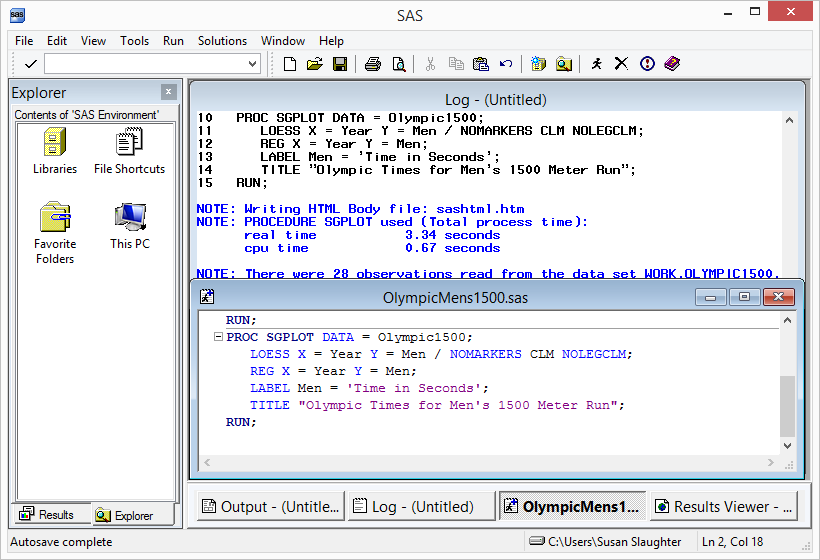
\includegraphics[scale=0.25]{sas9-4}
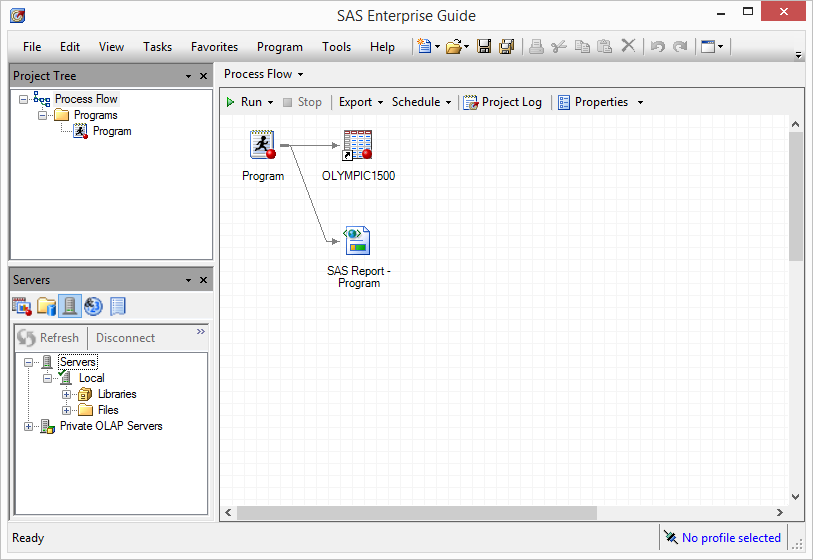
\includegraphics[scale=0.25]{sas-enterprise}
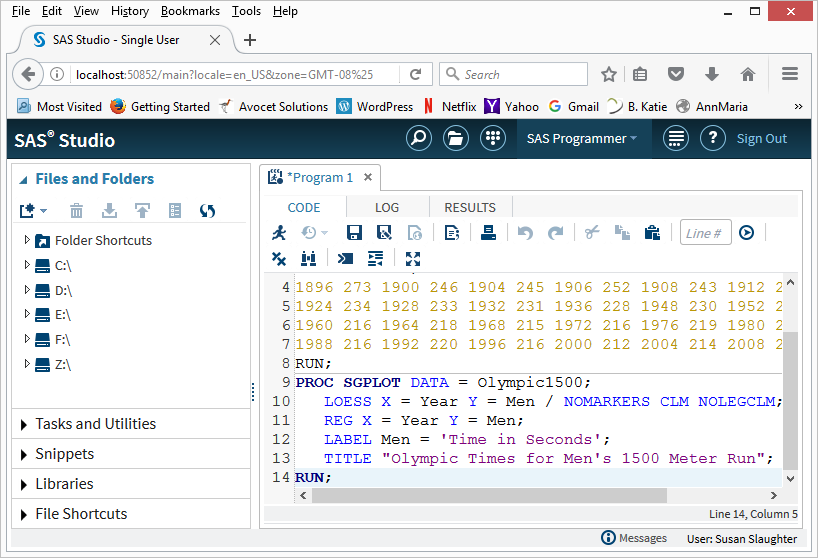
\includegraphics[scale=0.25]{sas-studio}
\caption{Captura de pantalla de los diferentes programas usados durante mis prácticas. De izquierda a derecha y de arriba a abajo: SAS 9.4, SAS Enterprise Guide y SAS Studio}
\label{fig:interfazSAS}
\end{center}
\end{figure}

En el inicio de las prácticas comencé usando SAS Studio ya que es el intérprete de SAS mas amigable con el usuario y es el que se usaba en el curso, aunque no el mas extendido por la empresa. Este programa nos permite realizar un tratamiento automático de los datos y realizar el análisis simplemente mediante la interfaz de usuario. 

Posteriormente, me enseñaron a usas SAS Enterprise Guide ya que era el que se usaba mas en la empresa. Es un programa muy similar a SAS Studio aunque te permite acceder al código generado y poder modificarlo. Aunque no tanto como SAS 9.4, este programa es que usé durante la mayoría de mi estancia en prácticas debido a que es el programa que es mas configurable y para el que estaban escritas la mayoría de las macros en la empresa. A pesar de no ser un programa tan \textit{user friendly} y no poder diseñar mediante la interfaz de usuario la \textit{pipeline} para procesamiento de los datos se podía hacer escribiendo código. De esta forma fue como más aprendí de SAS y su funcionamiento. 

Y finalmente SAS Viya fue usado al final de mi estancia en prácticas ya que la librería que se usaría para crear el nomograma estaba hecha para interactuar con SASViya. Aunque este software tiene una infinitud de posibilidades. 

Los \textbf{nomogramas} son unas representación gráfica que permite realizar con rapidez cálculos numéricos aproximados. Existen muchos tipos de nomogramas pero en mi caso el que usé fue un nomograma logístico. Esta clase de nomogramas son usado para poder realizar los cálculos de una regresión logística de manera aproximada, como el que se puede ver en la figura \ref{fig:nomograma}. Actualmente  los nomogramas son muy usados en el ámbito médico, para representar los riesgos de los pacientes a sufrir un cierto suceso, mostrándoles como actúa cada característica que presenta. Esto ayuda a que los pacientes asimilen mejor la información y no simplemente un número sino un proceso.  


\begin{figure}
\begin{center}
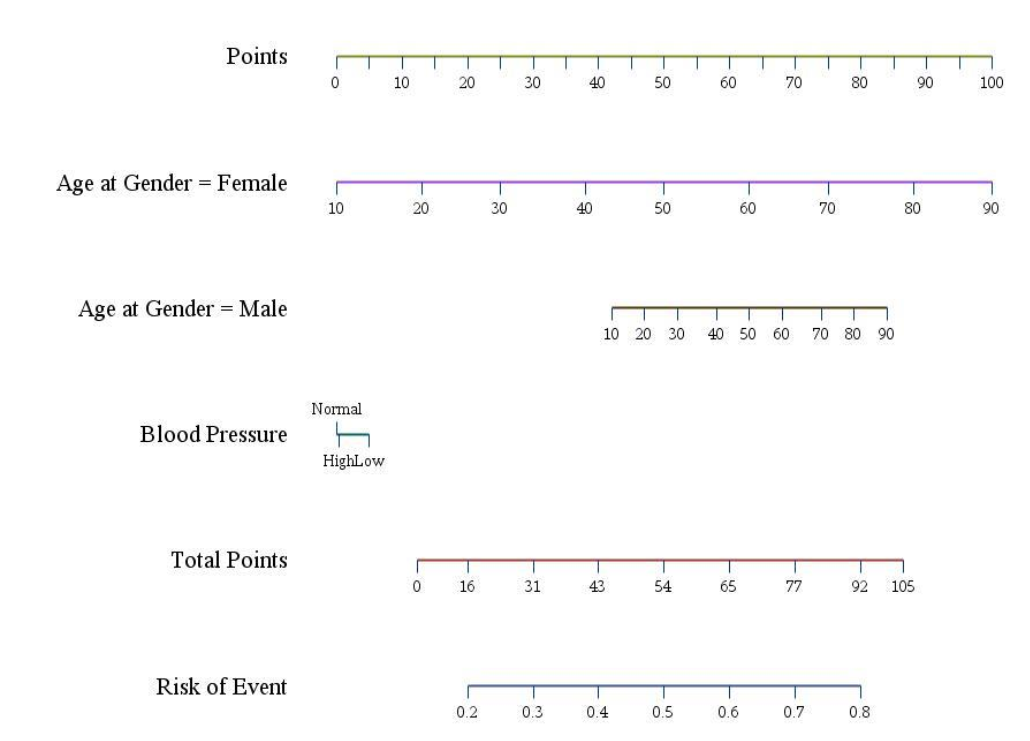
\includegraphics[scale=0.35]{ejemplo_nomograma.png}
\caption{Imagen de un nomograma de ejemplo realizado con SAS.}
\label{fig:nomograma}
\end{center}
\end{figure}

Además, para la realización del nomograma se usó el lenguaje de programación SAS y Python las librerías Pandas, para el manejo de las tablas en Python, y SASpy, permite la interconexión entre un servidor SAS y Python pudiendo así correr código de SAS en Python y obteniendo una sinergia casi perfecta entre las posibilidades que tiene SAS y la simplicidad de Python. 


\subsection{Etapas del desarrollo de las prácticas}

En el inicio de las prácticas se me asignó al grupo dirigido por Ana Gentil, Bussines Intelligence, al que asistía a las reuniones de grupo y ayudaba en diferentes tareas a los miembros de este. Durante este primer mes estuve realizando los cursos de SAS Programming 1 y 2 y el curso de IT de la empresa impartido por Felix Vidondo. Durante este periodo se me encargó la realización de un análisis estadístico para la doctora Infante de la unidad de Hematología del Hospital Universitario Infanta Leonor. Este proyecto sería la guía durante toda mi estancia en prácticas. El primer paso en cualquier proyecto de ciencia de datos es el tratamiento de los datos, que consiste en la clasificación de las variables, detección de nulos y outliers, detectar posibles fallos en la carga de los datos, asignación de etiquetas identificativas de cada variable \ldots Una vez se ha realizado un limpieza de los datos y el primer análisis exploratorio realicé un informe con los análisis de los datos para la doctora Infante.  

En este momento propuse a Carlos Goetz la realización de una macro que sacara el texto en \latex en vez de en Word que nos ahorrara tiempo a la hora de realizar los informes, esto es debido a en Word hacer la numeración de las imágenes debe de hacerse a mano además de poner el color de los textos a mano y estos problemas en \latex se solucionarían.  


Durante mi segundo mes en la empresa se me introdujo el proyecto de los doctores Blanca y Somoza del área de alergología del Hospital Universitario Infanta Leonor. Consistía en hacer un informe del análisis estadístico de los datos que nos había facilitado y posteriormente encontrar las mejores variables para realizar una regresión logística para predecir si un paciente sería hospitalizado o no. La primera parte del trabajo fue importar los datos y dar formatos a las variables y posteriormente realizar el análisis exploratorio y la realización del informe. Durante la realización de este informe se me introdujo al programa de recogida de datos médicos Red Cap. Este software sirve para el diseño de formularios para la recogida de datos en estudios médicos.
Una vez que se le entregó el informe del análisis estadístico a la doctora Infante tuvimos con ella y nos encargó  el cálculo la incidencia sobre los pacientes que necesitaron hospitalización y hacer un gráfico \textit{Swimmer plot}, como el que se puede observar en la figura \ref{fig:swimmerplot}, clasificando los pacientes según su tipo de infección y mostrar la duración del episodio infeccioso. 
\begin{figure}
\begin{center}
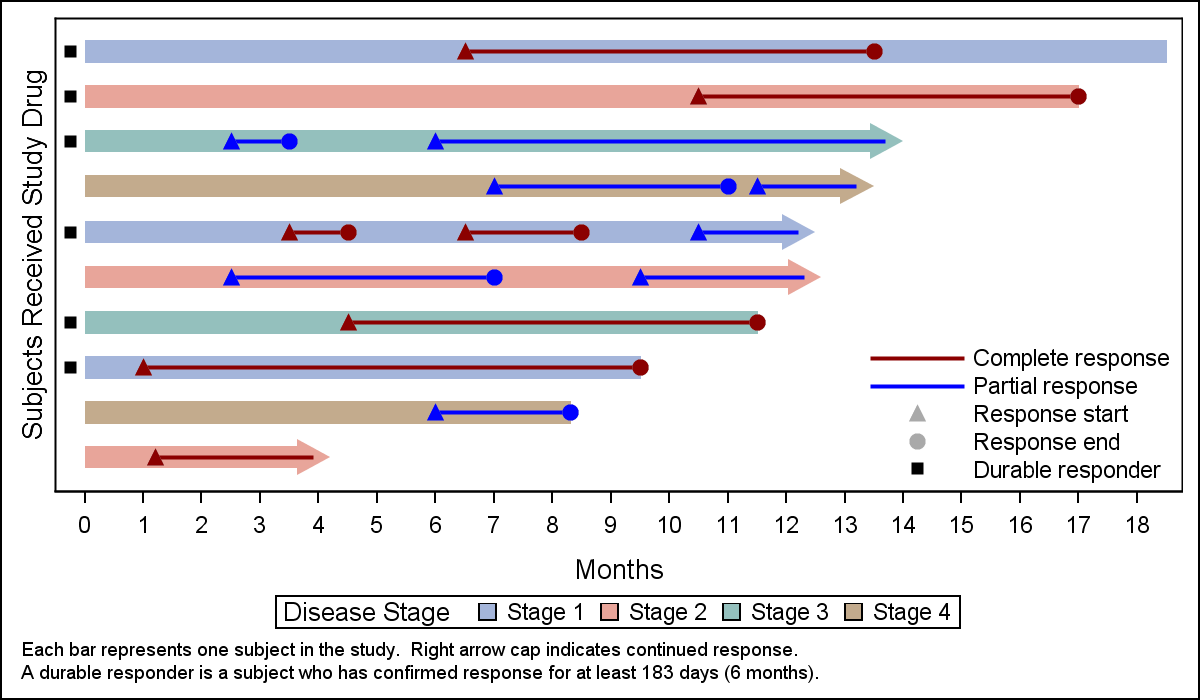
\includegraphics[scale=0.35]{swimmer_plot.png}
\caption{Imagen de un swimmer plot de ejemplo realizado con SAS.}
\label{fig:swimmerplot}
\end{center}
\end{figure}

En el tercer mes de prácticas debido a las fiestas de navidad y la tormenta Filomena que azotó la península ibérica las prácticas fueron en formato online y posteriormente siguieron debido a que tuve los exámenes finales. Durante este mes los días antes de Navidad estuve ayudando en el área de Bussines Intelligence con un proyecto que tenían y necesitaban ayuda. 
Posteriormente, se nos encargó en el grupo de Life Science la realización de un nomograma logístico automático siguiendo como esquema el artículo escirto por Dongsheng Yang. Este cambio en mi proyecto formativo fue debido a que muchos médicos les estaban pidiendo una forma visual de enseñar a sus pacientes porqué tienen un cierto riesgo y esta es la mejor forma de poder enseñarlo y la realización de un nomograma es muy larga, entonces se intentó automatizar este proceso. A la par que continué con mi formación realizando el curso de SQL y de Redes Neuronales en SAS. \cite{nomograma}


Durante el último mes continué con la realización de la creación de nomogramas automáticos mediante SAS. Pero al ver que no podía avanzar utilizando el lenguaje de programación de la empresa comencé a utilizar Python con la librería SASPy. Consiguiendo así un buena sinergia entre la flexibilidad de de Python y la potencia en cálculo estadístico de SAS. Finalmente, conseguí alcanzar  el objetivo de la realización de un nomograma automático, un ejemplo de la salida de este programa se puede observar en la figura \ref{fig:nomogramaSASpy}, y el código se puede encontrar en el Anexo \ref{anexo:codigonomograma}.
Durante este ultimo mes escribí dos artículos a la ''wiki'' de la empresa, wikiPeRTICA. En ellos expliqué como se debía instalar SASpy y como usar sus diferentes funciones y como utilizar el programa habia hecho.

\begin{figure}
\begin{center}
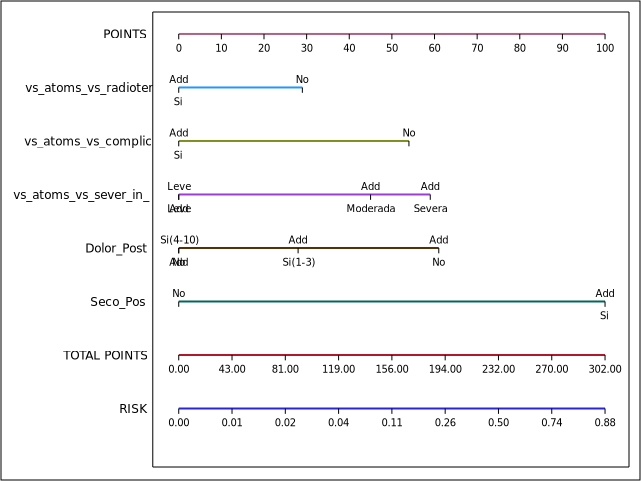
\includegraphics[scale=0.45]{SVG.png}
\caption{Imagen de un nomograma de ejemplo realizado con SASpy.}
\label{fig:nomogramaSASpy}
\end{center}
\end{figure}


\section{Conclusiones y valoración personal}
Gracias a estas prácticas he podido afianzar ciertos conocimientos que he aprendido durante la carrera en las diversas asignaturas de estadística y probabilidad. Además, de poder aprender un nuevo lenguaje de programación como es SAS y poder mejorar mi manejo de Python  asi mismo aprender nuevas librería como pueden ser Pandas y SASpy. Sin menospreciar el conocimiento que he adquirido sobre algoritmos de clasificación supervisada, como pueden ser la regresión logística, y en regresiones logísticas . 

Estas prácticas me han ayudado a introducirme en el mundo laboral de una manera muy buena, debido a que he podido ver los diferentes ámbitos de la ciencia de datos y todos los pasos que hay en el proceso de un proyecto. Aunque no he podido ver a fondo la parte de los planes de proyecto y como realizar la administración de los recursos. 
Además, estoy muy agradecido a Carlos y Juan por la libertad a la hora de  elegir la estrategia para solucionar los problema y poder investigar nuevas soluciones.

\chapter{Memoria TFG}

\section {Introducción}



\section{Conceptos previos}

En esta sección se van a mostrar algunos conceptos previos que van a ser necesarios para poder entender este trabajo. Primero explicaremos algunos conceptos básicos sobre álgebra lineal y posteriormente  se explicarán algunos conceptos sobre los tensores. 

\subsection{Conceptos básicos}
\begin{defi}[Ver \cite{Fomenko}]
Sea $\varphi:$\M $\to$ \M' una homeomorfismo entre dos variedades. Decimos que $\varphi$ es un \textbf{difeomorfismo} si la inversa es diferenciable. Y diremos que es de clase $\mathscr{C}^r$ si es r veces diferenciable. 
\end{defi}


\begin{defi}[Ver\cite{Fomenko}] 
Decimos que $(U, \varphi)$ y $(V, \psi)$ son  \Cinf -compatibles si $U \cap V \neq \emptyset$ implica que $\varphi \circ \psi^{-1} $ y $ \psi \circ \varphi^{-1}$ son difeomorfismos de los abiertos $\varphi(U \cap V )$ y $\psi(U \cap V )$ de \R$^n$.C
\end{defi}

\subsection{Conceptos básicos de álgebra lineal}
\begin{defi}[Ver \cite{algebralineal}]
Sea V un espacio vectorial sobre un cuerpo K. El \textbf{espacio vectorial dual} de V es el conjunto de todas las aplicaciones lineales $\varphi :V \to K$. Y se denotará como $V^*$.
Y a los elementos de $V^*$ se les llamará covectores o uno formas. 
También se le puede denotar como $Hom_k(V,K)$.
\end{defi}

\begin{defi}[Ver \cite{algebralineal}]
Sea V un K-espacio vectorial y sea $V^*$ el dual. Diremos que $\beta = {e^i}_{i=1}^n$ una base de V, entonces la base dual asociada a $\beta$, $\beta^* = {e_i^*}_{i=1}^n$, cumplirá que 
$\forall i\ j \ e^*_j e^i = \delta_i^j$ 
\end{defi}


\begin{defi}[Ver \cite{algebralineal}]
Una \textbf{aplicación multilineal} o formas multilineales, es una aplicación de un espacio vectorial, $V^n$, a un cuerpo K, de dimensión m. 
\begin{center}
$ f:V^n \to K$

$(v_1, \ldots, v_n) \to f((v_1, \ldots, v_n))= (f_1((v_1, \ldots, v_n)), \ldots, f_m((v_1, \ldots, v_n) ) )$
\end{center}
Y para cada $f_i$ será una aplicación lineal. 
Diremos que una forma multilineal es: 
\begin{itemize}
    \item \textbf{definida positiva} si $\forall \x \in V f \x \geq 0$ 
    \item \textbf{no degenerada} si $f(\x) = 0$ si y solamente si $\x = \vec{0}$
    
\end{itemize}
\end{defi}


\subsubsection{Tensores}
En esta subseción se van a mostrar conceptos básicos sobre los tensores. 

\begin{defi}[Ver \cite{chamizo}]
    Sea V un espacio vectorial real. Un \textbf{tensor n veces covariante} es cualquier aplicación multilineal $T:\times_{i=1}^n V \to $\R. Al conjunto de todos los k-tensores se denota como $\mathcal{T}^k(\mathscr{M})$
\end{defi}

\begin{ejem}
Para visualizar esto vamos a poner el ejemplo de un determinante de una matriz 3x3. 
$$\begin{array}{l}
T: \mathbb{R}^{3} \times \mathbb{R}^{3} \times \mathbb{R}^{3} \longmapsto \mathbb{R} \\
T \left( \left(\begin{array}{l}
x_{1} \\
x_{2} \\
x_{3}
\end{array}\right),\left(\begin{array}{l}
y_{1} \\
y_{2} \\
y_{3}
\end{array}\right)\left(\begin{array}{l}
z_{1} \\
z_{2} \\
z_{3}
\end{array}\right)\right) \longmapsto\left|\begin{array}{lll}
x_{1} & y_{1} & z_{1} \\
x_{2} & y_{2} & z_{2} \\
x_{3} & y_{3} & z_{3}
\end{array}\right| 
\end{array}  $$

La propiedad de producto por un escalar se deduce se realizar el desarrollo por adjuntos por columnas y observar que se puede sacar factor común el escalar. 

La propiedad de linealidad se deduce también de realizar el desarrollo por adjuntos. 
\end{ejem}

\begin{defi}[Ver \cite{chamizo}]
Sea V un espacio vectorial real de dimensión n, y sea $V^*$ su espacio dual. Definiremos un \textbf{tensor r veces contravariante} a una aplicación multilineal $T: \times_{ i = 1}^n V^*\to \mathbb{R}
$
\end{defi}


\begin{defi}[Ver \cite{chamizo}]
Sea V un espacio vectorial real y sea $V^*$ su espacio vectorial dual. Entonces, un \textbf{ tensor r veces contravariante y s veces covariante} será una aplicación multilineal de la forma: \end{defi}
\begin{equation*}
    T:\times_{i=1}^r V^* \times \times_{j=1}^s V \to \mathbb{R}
\end{equation*}
Y se denotara como un tensor de tipo (r,s).


\begin{propo}[Ver \cite{chamizo}]
Toda aplicación multilineal del tipo $T:\times_{i=1}^nV \to \mathbb{R}^m
$ se puede transformar a un tensor de tipo  $T:\times_{i=1}^nV \to \mathbb{R}
$ mediante el uso de elementos del espacio dual.
\end{propo}

\begin{defi}[Ver \cite{gondinho}]
Dados dos tensores T y S de rangos k y m, entonces se define el \textbf{tensor producto} como el tensor (k+m)-tensor dado por: 
\begin{equation*}
    T\otimes S(v_1,\ldots,v_k,v_{k+1},\ldots, v_{k+m}):= T(v_1,\ldots,v_k)\times S(v_{k+1},\ldots, v_{k+m})
\end{equation*}\cite{gondinho}
\end{defi}

\begin{defi}[Ver \cite{gondinho}]
Sea \M una variedad diferenciable y sea T un tensor de tipo (0,s) en \M. entonces podemos definir un nuevo tensor llamado \textbf{Alt(T)}  de la siguiente manera:
\begin{equation*}
    Alt(T) :=\frac{1}{k!} \sum_{\sigma \in S_n} sgn(\sigma)(T\circ \sigma) 
\end{equation*}
Con $S_n$ el conjunto de todas las permutaciones de n elementos y \textit{sgn} la signatura de la permutación.
\end{defi}

Y ahora definimos el \textbf{producto cuña } y lo denotaremos como $\bigwedge$ de dos tensores T y S de clase (0,n) y (0,m) a: 
\begin{equation*}
    T \wedge  S := \frac{(n+m)!}{n! m!} Alt(T\otimes S)
\end{equation*}

\section{Variedades diferenciables}
Para poder comenzar el estudio de las geodésicas vamos a necesitar una ''superficie'' en la que se encuentre. Pero vamos a necesitar una generalización de las   ''superficies'' a dimensiones mayores y a conjuntos en los que no hay casi ninguna estructura matemática definida sobre ellos.
A estas generalizaciones las vamos a llamar variedades. Las más básicas son las variedades topológicas, están definidas sobre espacios topológicos únicamente, y deben de cumplir una serie de proposiciones, como vamos a ver en la siguiente definición.

\begin{defi}[Ver \cite{boothby}]
Una \textbf{variedad} ó \textbf{variedad topológica} $\mathcal{M}$ de dimensión n, ó una n-variedad, es un espacio topológico con las siguientes propiedades:
\begin{enumerate}
\item \M es Hausdorff.
\item \M es localmente euclídeo de dimensión n. \footnote{Para todo $p \in$  \M existe un entorno \U de p tal que $\exists \varphi: U' \subseteq $\R$^n \to $\U  que es un homeomorfismo}
\item \M satisface el segundo axioma de numerabilidad, es 2AN.
\end{enumerate}
\label{def:variedad_topo}

\end{defi}

Pero para poder operar sobre estas variedades topológicas vamos a necesitar que estas estén equipadas con algunos objetos matemáticos. Si a una variedad topológica se le dota de una estructura diferenciable, es decir, un conjunto de aplicaciones continuas, inyectivas y diferenciables de \R$^n$ a nuestra variedad, \M. Esta variedad dotada de una estructura diferenciable cumple una serie de proposiciones diremos que es una variedad diferenciable, como vamos a ver en la siguiente definición.


\begin{defi}[Ver \cite{DoCarmoRiemann}]
Si una variedad topológica, \M, es dotada de una estructura diferenciable, es decir, un conjunto de aplicaciones inyectivas $X = \lbrace$ $ x_\alpha : U_\alpha \subset $\R$^n \rightarrow M $ tal que $U_\alpha \subset $\R$^n$ es un abierto  $\rbrace_{\alpha \in I}$. Y si cumple las siguientes proposiciones diremos que es una \textbf{variedad diferenciable} si:
 \begin{enumerate}
 \item $\bigcup_{\alpha\in I} \textbf{x}_\alpha(U_\alpha) = M $
 \item $\forall \ \alpha , \beta \in I $ con $x_\alpha(U_\alpha) \bigcap x_\beta(U_\beta) = W \neq \emptyset $ por lo cual
 $ x_\alpha^{-1}(W) \ y \  x_\beta^{-1}(W) $ son conjuntos abierto en \R$^n$ y la aplicación $x_\beta^{-1}\circ x_\alpha $ es diferenciable. (Fig:\ref{Fig:Variedad})
 \item La familia $\lbrace(U_\alpha, \textbf{x}_\alpha)\rbrace_{\alpha \in I}$ es maximal relativa a las condiciones 1. y 2.
\end{enumerate} 
 Lo que enuncia 3. es que si se tiene una estructura diferencial $\mathscr{V} =\{ (U_i, \textbf{x}_i) \}_{i \in I}$ de \M y una parametrización ($U_0, \textbf{x}_0$) de \M tal que $\textbf{x}_0^{-1} \circ \textbf{x}_i $ y $\textbf{x}^{-1}_i \circ \textbf{x}_0$ es de clase \Cinf para todo  $\textbf{x}_i$ de  $\mathscr{V}$ entonces ocurre que  ($U_0, \textbf{x}_0$) pertenece a  $\mathscr{V}$.
 
A cualquier familia $\lbrace U_i, \textbf{x}_i \rbrace_{i \in I} $ que satisface las dos primera proposiciones de la definición anterior se le llama \textbf{atlas} de \M y si también satisface la tercera proposición  se le llamará \textbf{atlas maximal}.
\label{def:variedad_dif}
\end{defi}

Puede ocurrir que una variedad no tenga ninguna estructura diferenciable compatible o que tenga varias. En este último caso diremos que dos atlas son  \textbf{equivalentes} si ambos definen las misma estructura diferenciable. 

\begin{figure}[!ht]
\centering
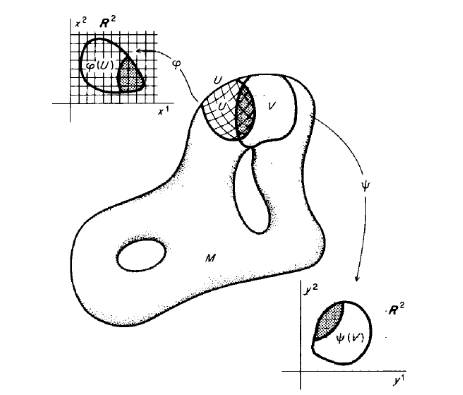
\includegraphics[scale=0.5]{ImagenBonitaVariedad.png}
\label{Fig:Variedad}
\caption{ Parametrización e intersección de sus imágenes.\cite{boothby}}
\end{figure}

Para poder ilustrar el ejemplo de una variedad vamos a mostrar que una esfera n-dimensional es una variedad n-dimensional.
\begin{ejem}[Ver \cite{Fomenko}] 
Sea $\mathcal{S}^n \subset $\R$^{n+1} $ tal que $\mathcal{S}^n = \lbrace \vec{x} \in \mathcal{S}^n \therefore \|\vec{x}\| = 1\rbrace  $.\\
Se definen los abiertos coordenados de \R$^n$ como:\\
$$ U^+_i = \lbrace \vec{x} =  (x_1,\dots, x_i, \dots , x_n) \in \s^n \therefore x_i > 0 \rbrace $$\\
$$ U^-_i = \lbrace \vec{x} =  (x_1, \dots, x_i, ... , x_n) \in \s^n \therefore x_i < 0 \rbrace $$\\
Por consiguiente que para todo punto de $\s^n$ pertenecerá a las cartas $ U^+_i $ ó $U^-_i$. De manera que se tendrá que 2I + 2 cartas que satisficieran el primer requisito. 
$$ \s^n \subset \bigcup_{i = 0}^I U^+_i \cup \bigcup_{i = 0}^I U^-_i  $$

Después, se buscan los homeomorfismos coordenados. Que cumplan la segunda propiedad de la definición \ref{def:variedad_dif}.
$ \textbf{x}_i^{-} = \textbf{x}_i^{+} : U_i \subseteq$ \R$^{n+1} \rightarrow$ \R$^n$
$$ (x_0,\dots, x_n) \rightarrow \textbf{x}_i (x_0,\dots, x_n) = (x_0,\dots,x_{i-1}, x_{i+1}, \dots, x_n)$$
Como se  observa es la proyección i-ésima de \R$^{n+1}$ a \R$^n$. Que como bien se ha visto en la asignatura de topología es continua. Ahora falta ver que son biyectivas, para ello se va demostrar que es suprayectiva e inyectiva.\\

Y los homeomorfismos inversos son:\\
\begin{equation}
    \begin{aligned}
        (\textbf{x}_i^+)^{-1} (x_1,\dots, x_n) = (x_0,\dots,x_{i-1},\sqrt{1-(x_1^2+\dots +x_n^2)} , x_{i+1}, \dots, x_n) \\
(\textbf{x}_i^-)^{-1} (x_1,\dots, x_n) = (x_0,\dots,x_{i-1},-\sqrt{1-(x_1^2+\dots+ x_n^2)} , x_{i+1}, \dots, x_n)   
    \end{aligned}
\end{equation}

Como podemos ver estas funciones son continuas. 

\end{ejem}

Similar a como ocurre en \R$^3$ en las variedades también existen espacios tangentes a un punto.
Si recordamos el concepto de plano tangente a un punto p de una superficie es el conjunto de vectores que son tangentes a la superficie en el punto, pero en el caso de las variedades el concepto de vector tangente no está definido por ello es necesario introducirlo. 

\begin{defi}
Se define el concepto de \textbf{$\mathscr{C}^\infty$(p)} como el conjunto de todas las aplicaciones $f:\mathscr{M} \to \mathbb{R}$  tales que existe la derivada de \f  en el punto p.
\end{defi}

\begin{defi}[Ver \cite{DoCarmoRiemann}]
Sea \M una variedad n-dimensional, sea $\alpha:$]$-\varepsilon, \varepsilon$ [ $\to$ \M  diferenciable y $\alpha (0) = p \in$\M tal que $\alpha(t) = (x_1(t), ...,x_n(t))$ y  $\dot{\alpha}(0) = (\dot{x_1}(0), ...,\dot{x_n}(0))= \vec{v}$ y sea $f$ $\in$ \Cinf(p). Definimos \textbf{vector tangente de $\alpha$ en p}, se denota $\dot{\alpha}(f)$, como la restricción de la derivada direccional de $f$ con respecto a $\vec{v}$:
\begin{equation}
\frac{ d(f \circ \alpha)}{dt}\bigg|_{t=0} = \sum_{i=0}^{n} \frac{\partial f}{\partial x_i}\bigg|_{t=0} \frac{d (x_i)}{dt}\bigg|_{t=0} = \sum_{i=0}^{n} \dot{x}_i(0)\frac{\partial f}{\partial x_i}\bigg|_{t=0} = 
 \bigg(\sum_{i=0}^{n} \dot{x}_i(0)\frac{\partial }{\partial x_i}\bigg|_{t=0}\bigg)f
\end{equation}
Y se puede observar que el vector tangente de $\alpha$ en p solamente depende del vector $\vec{v}$. 
\end{defi}

\begin{propo}\label{cambio_componentes}
[Ver \cite{WinterSchool}]
Se \M una variedad diferenciable y sean \{U,$\phi$\} y \{V,$\psi$\} dos cartas de \M, y sea $p \in \phi(U)\cap \psi(V) $. Y sea $x \in $\tpm entonces x respecto de  las cartas $x_\phi = \sum_i x_\phi^i \frac{\partial}{\partial \phi_i}\bigg|_{p} $ y $x_\psi =\sum_i x_\psi^i \frac{\partial}{\partial \psi_i}\bigg|_{p} $.

¿Cómo estan realcionados $\{\x_\psi^i \} y \{x_\phi^i \} $?
Sea $f \in C^\infty(p) $. Para simplificar la notación denotaremos de esta forma: (Criterio de suma de Einstein )
\begin{equation}
    \begin{aligned}
           \frac{\partial}{\partial \phi_i}\bigg|_p (f)= \partial_i(f\circ \phi^{-1})(p) \\ 
   \frac{\partial }{\partial \psi_i }\bigg|_p (f)= \partial_i(f \circ \psi^{-1})(\psi(p)) 
    \end{aligned}
\end{equation}

Entonces:
\begin{equation}
 \begin{aligned}
      \partial_i(f\circ \phi^{-1})(p) = & \partial_i(f\circ \psi^{-1} \circ \psi  \circ \phi^{-1})(p) \\
     =& \partial_i(f \circ \psi^{-1})\bigg|_{\psi(p)}\partial_j(\psi \circ \phi^{-1} )\bigg|_{\phi(p)}\\
     =& \frac{\partial f}{\partial \psi^j}\bigg|_p\frac{\partial \psi^j}{\partial \phi^i}\bigg|_p \\
     =&\frac{\partial \psi^j}{\partial \phi^i}\bigg|_p\frac{\partial }{\partial \psi^j}\bigg|_p(f) 
\end{aligned}   
\end{equation}


Entonces, $x_{\phi}^j =\frac{\partial \psi^j}{\partial \phi^i}\bigg|_p \frac{\partial }{\partial \psi^j}\bigg|_p $ y finalmente obtenemos que $x_\psi^j = x_\phi^i \frac{\partial \psi^j}{\partial \phi^i} \bigg|_p = \partial_i(\phi)$ 
\end{propo}

Una vez se ha definido el concepto de vector tangente de $\alpha$ en p y hemos visto como varía respecto de un cambio de cartas podemos definir ya el espacio tangente a una variedad diferencial en el punto p de una manera muy similar al caso de \R$^3$.

\begin{defi} [Ver \cite{DoCarmoRiemann}]
Sea \M una variedad diferencial n-dimensional, y sea $\alpha$ una curva diferenciable de \M tal que $\alpha(0)= p \in$ \M . Entonces se define el \textbf{espacio tangente de \M en p}, y se denota \tpm, como: 
\begin{equation}
   T_p\mathscr{M}= \{\dot{\alpha}(f)\therefore f \in \mathscr{C}^\infty(p)\ y \ \frac{d \alpha}{dt} \neq 0 \ tal \ que \  \alpha(0)=0\}
\end{equation}
\end{defi}

\begin{defi}[Ver \cite{WinterSchool}]
Al espacio dual de \tpm se le llamará espacio cotangente, y se denotará como \tpm$^*$. Y será:
\begin{center}
    \tpm$^*:=\{\varphi:$ \tpm$ \to$\R $: \varphi \text{es una aplicación lineal}  \}$
\end{center}
Una base del espacio cotangente respecto de la carta \{U,x\} será $d(x_i)_p$.
\end{defi}

\begin{figure}[!ht]
\centering
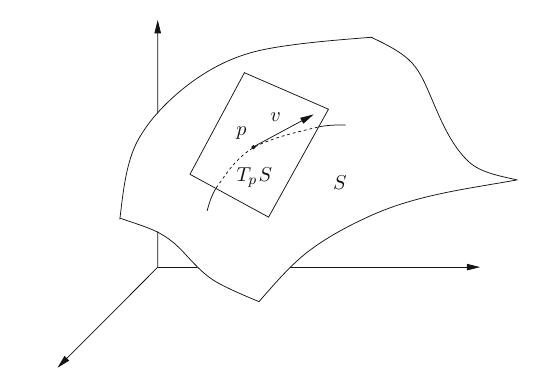
\includegraphics[scale=0.5]{imagenTpS.png}
\label{Fig:TpS}
\caption{ Espacio tangente de una superficie.\cite{gondinho}}
\end{figure}
\newpage

Pero esta idea tan abstracta de vector tangente en un punto no es muy operativa. Para poder manejar este concepto vamos a usar los atlas de la variedad ya que nos transportan nuestra variedad a un objeto de \R$^n$ que si que conocemos bien. Para poder operar con ello vamos a necesitar una parametrización de $ \mathscr{V} \subseteq$\M, con $p \in \mathscr{V} $, $\varphi : U\subseteq $\R$^n \rightarrow  \mathscr{V} \subseteq$ \M \  tal que $\varphi (0)= p$ y sean $f \in \mathscr{C}^\infty$(p) y la curva $c:]-\varepsilon, \varepsilon[ \rightarrow$ \M una curva diferenciable tal que $\alpha(0)=p$. Definamos:\\

\begin{center}
 $\dot{c}$:= $[\varphi^{-1} \circ c](t)=(x^1(t),\ldots, x^n(t))$ 
\end{center}
Entonces:\\
$$\dot{c}(0)(f)= \frac{d(f \circ c)}{dt}(t)\bigg|_{t=0} = \frac{d((f\circ \varphi) \circ (\varphi^{-1}\circ c)))}{dt}\bigg|_{t=0}$$
Por simplificar la notación denotemos $f\circ \varphi$ como \^{f} y a $ \varphi^{-1}\circ c)$ como $\hat{c}$.
\begin{equation}
    \begin{aligned}
           \dot{c}(0)(f) = & \frac{d(\hat{f}\circ \hat{c})}{dt}\bigg|_{t= 0} =
           \sum_i \frac{\partial(\hat{f})}{\partial(x^i)}\bigg|_{\hat{c}(0)} 
           \frac{d(x^i(t)}{dt}\bigg|_{t=0} \\
           = & \sum_i   \frac{\partial(\hat{f})}{\partial(x^i)}\bigg|_{\varphi^{-1}(p)}\dot{x}^i(0) \bigg[\sum_i \frac{\partial}{\partial(x^i)}\bigg|_{\varphi^{-1}(p)} \dot{x}^i(0)\bigg](\hat{f})
    \end{aligned}
\end{equation}


Siendo $\frac{\partial}{\partial(x^i)}\bigg|_{\varphi^{-1}(p)}$ el vector tangente a p de la curva en la dirección $x^i$

Entonces, el vector $\dot{c}(0)$ se puede expresar respecto de la parametrización $\varphi$ como:
\begin{center}
$\dot{c}(0) = \sum_i \frac{\partial}{\partial(x^i)}\bigg|_{\varphi^{-1}(p)} \dot{x}^i(0) $
\end{center}


\begin{propo}[Ver \cite{WinterSchool}]
El espacio tangente en un punto es un espacio vectorial de dimensión n. Y su base será$\lbrace \frac{\partial}{\partial x^i} \rbrace_{i = 1}^n$.
\end{propo}
\bproof
Primero vamos a demostrar que \tpm es un espacio vectorial. Y después, que  $\lbrace \frac{\partial}{\partial x^i} \rbrace_{i = 1}^n$ es una base de \tpm .

Por simplicidad a los elementos de \tpm los denotaremos como $v_{\gamma, p}$

Para demostrar que es un $\mathbb{R}$ espacio vectorial primero definiremos las dos operaciones necesarias $\oplus, \otimes$ tales que: 
\begin{center}
	$\oplus: T_p\mathscr{M} \times T_p\mathscr{M} \to T_p\mathscr{M}$\\
		$v_{\gamma,p}\oplus v_{\alpha, p}(f) \to v_{\gamma,p}(f) \oplus v_{\alpha, p}(f)$ \\
\end{center}
\begin{center}
	$\otimes: \mathds{R} \times T_p\mathscr{M}  \to T_p\mathscr{M} $ \\
		$\lambda \otimes v_{\gamma,p}(f) \to \alpha v_{\gamma,p}(f)$ 
\end{center}
Con $\gamma(\lambda_0) = p$ y $\alpha(\lambda_1) = p$.


Vamos a demostrar que son operaciones cerradas. Primero demostramos que $\otimes$ es cerrado: 
\\Sea $\tau :$\R$  \to M$ tal que $\lambda \to \tau(\lambda) := \gamma(\alpha \lambda + \lambda_0)$ Para simplificar tomamos vamos a denotar a  $\alpha \lambda + \lambda_0$ como $\nu_\alpha$ entonces queda de la forma $ \tau(\lambda) := \gamma\circ \nu_\alpha(\lambda)$

Y vamos a ver que es una curva de \tpm , ya que $\tau(0) = \gamma(\lambda_0) = p$ y vamos a ver el vector tangente: 
\begin{center}
$v_{\tau, p} = \frac{d(f \circ \tau)}{dt}\bigg|_{t= 0} = \frac{d(f\circ \gamma \circ \nu_\alpha)}{dt}\bigg|_0 = \frac{d(f\circ \gamma)}{dt}\bigg|_{t=\lambda_0} \frac{d(\nu_\alpha)}{dt}\bigg|_{t=0} = \alpha \frac{d(f\circ \gamma)}{dt}\bigg|_{t = \lambda_0} \in$ \tpm
\end{center}

Y ahora vamos a ver que es $\oplus$ genera elementos de \tpm . Para demostrarlo tomaremos una carta \{U, x\}, y al final demostraremos que no depende de dicha carta a riesgo de perder generalidad pero llegaremos a que no depende de esta.

Sea $\sigma_x :$\R $\to M$ tal que $\sigma_x(\lambda) := x^{-1}((x\circ \lambda)(\lambda_0 + \lambda) + (x \circ \alpha)(\lambda_1 + \lambda) - (x \circ \gamma)(\lambda_0))$ 

Que va a satisfacer que:
\begin{itemize}
	\item $\sigma_x(0) =x^{-1}((x\circ \lambda)(\lambda_0 ) + (x \circ \alpha)(\lambda_1 ) - (x \circ \gamma)(\lambda_0)) = x^{-1}((x \circ \alpha)(\lambda_1 )) = \alpha(\lambda_1) = p $ 
	\item  	Y que $\sigma_x \in$ \tpm entonces: 


\begin{equation}
    \begin{aligned}
       v_{\sigma_x, p} =& \frac{d(f\circ \sigma_x)}{dt}\bigg|_{t=0} \\
       =& \frac{d(f\circ x^{-1} \circ x \circ \sigma_x)}{dt} \bigg|_{t=0} \\
       =& \sum_i \frac{d(x_i \circ \sigma_x)}{dt}\bigg|_{t=0} \frac{\partial(f \circ x_i^{-1})}{\partial x_i}\bigg|_{x(\sigma_x(0))}\\
       =&\sum_i \bigg[\frac{d(x_i \circ \gamma)}{dt}\bigg|_{\lambda_0} + \frac{d(x_i \circ \alpha)}{dt}\bigg|_{\lambda_1} \bigg] \frac{\partial(f \circ x_i^{-1})}{\partial x_i}\bigg|_{x(\sigma_x(0))}\\
       =& \bigg[ \frac{d(x_i \circ \gamma)}{dt}\bigg|_{\lambda_0} \frac{\partial(f \circ x_i^{-1})}{\partial x_i}\bigg|_{x(p)} \bigg] + \bigg[\frac{d(x_i \circ \alpha)}{dt}\bigg|_{\lambda_1}\frac{\partial(f \circ x_i^{-1})}{\partial x_i}\bigg|_{x(p)}\bigg] \\
       =& \frac{d(f \circ x^{-1} \circ x \circ \gamma )}{dt} \bigg|_{t=\lambda_0} + \frac{d(f \circ x^{-1} \circ x \circ \alpha)}{dt}\bigg|_{t=\lambda_1}\\
       =& \frac{d(f\circ \gamma)}{dt}\bigg|_{\lambda_0} + \frac{d(f \circ \alpha)}{dt}\bigg|_{\lambda_1}\\
       =& v_{\gamma,p} + v_{\alpha, p}\   \forall f \in \mathscr{C}^\infty(p)
    \end{aligned}
\end{equation}

 

	
Que ambos pertenecen a \tpm. 
\end{itemize}
 Por lo tanto hemos demostrado que $\oplus$ y $\otimes$ son operaciones válidas para \tpm . Entonces solamente quedaría probar que con estas dos operaciones \tpm es un espacio vectorial real. 


Ahora vamos a demostrar que  $\lbrace \frac{\partial}{\partial x^i}\bigg|_p \rbrace_{i = 1}^n$ es una base de \tpm respecto de la carta $\varphi = (x_1,\ldots, x_n)$. Para demostrar que es una base de este espacio vectorial vamos a demostrar que son linealmente independiente. 

Un conjunto de vectores son linealmente independientes si $\sum_i \lambda_i v_i = 0$ si y solo si $\forall \lambda_i = 0$
\begin{equation}
\begin{aligned}
    \sum_j \sum_i \lambda_i \frac{\partial}{\partial x^i} x^j = &0\\
\sum_j \sum_i \lambda_i \delta_i^j =&\\
\sum_i \lambda_i =&
\end{aligned}
\end{equation}
Por lo tanto $\lbrace \frac{\partial}{\partial x^i}\bigg|_p \rbrace_{i = 1}^n$ es una base de \tpm de dimensión n.
\eproof

\begin{defi}[Ver \cite{gondinho}]
Sea \M una variedad y sean \{U,x\} una carta de \M y $\gamma:$\R$\to U$ una curva sobre \M tal que $\gamma(0)=p$. Entonces la representación de $v_{\gamma,p}$ respecto de x será:
\begin{equation}
    \begin{aligned}
           v_{\gamma,p}=&  \frac{d(f \circ \gamma)}{dt}\bigg|_{t=0}\\
           =&\frac{d(f \circ x^{-1} \circ x \circ \gamma)}{dt}\bigg|_{t=0}\\
           =& \frac{d(x^i \circ \gamma)}{dt}\bigg|_{0} \frac{\partial f}{\partial x^i}\bigg|_{p}\\
            =& \dot{\gamma}_x^i\bigg|_0\frac{\partial }{\partial x^i}\bigg|_{p} (f)  
  \end{aligned}
\end{equation}
 
Y como hemos demostrado que $\lbrace \frac{\partial}{\partial x^i}\bigg|_p \rbrace_{i = 1}^n$ es una base de \tpm entonces $v_{\gamma,p}$ respecto de la carta x será $ \dot{\gamma}_x^i\bigg|_0 $
\end{defi}


Se dice que una variedad, \M de dimensión n, es \textbf{no degenerada} si para todo punto de \M  existe \tpm 

\begin{defi}[Ver \cite{gondinho}]
A la unión de todos los espacio es tangente de \M  se denota como T(\M): 
\begin{equation}
T(\mathscr{M})= \bigcup_{p \in \mathscr{M}} T_p \mathscr{M}
\end{equation}

A este espacio se le llama \textbf{fibrado tangente}. Y es posible dotarlo de una estructura diferenciable de dimensión 2n.

\end{defi}

Para poder visualizar esta idea de vector tangente a una variedad vamos a usar el ejemplo de la esfera de dimensión 2. 

\begin{ejem}[Ver \cite{gondinho}]
Sea la variedad $S^2$  y sea el punto Sea $p \in$ \M , con $p \neq (0,0,-1)$ y $p \neq (0,0,-1)$. Una parametrización de un entorno de dicho punto es:
\begin{equation}
    \begin{aligned}
           \varphi:(0, \pi)&\times(-\pi,\pi)\rightarrow S^2 \\ 
           \varphi(\theta, \psi)=& (cos(\theta)sin(\psi), sin(\theta)sin(\psi), cos(\psi))
    \end{aligned}
\end{equation}

Ahora vamos a sacar el espacio tangente a p. Que vendrá generado por $\beta = \lbrace \frac{\partial}{\partial \theta}\bigg|_{p},\frac{\partial}{\partial \psi}\bigg|_{p} \rbrace$
Entonces: 
\begin{equation}
    \begin{aligned}
           \frac{\partial \varphi}{\partial \theta}\bigg|_{p}=& (-sin(\theta)sin(\psi),cos(\theta)sin(\psi),0)\\
	\frac{\partial \varphi}{\partial \psi}\bigg|_{p} =& (cos(\psi)cos(\theta),cos(\psi)sin(\theta),-sin(\psi))
    \end{aligned}
\end{equation}

Y obtenemos la base $\beta$ respecto de la parametrización $\varphi$: 
\begin{center}
	$\beta= <\lbrace (-sin(\theta)sin(\psi),cos(\theta)sin(\psi),0) , (cos(\psi)cos(\theta),cos(\psi)sin(\theta),-sin(\psi))\rbrace>$
\end{center}

\end{ejem}




\section{$\mathbb{R}^n$ como variedad}
A partir de este momento tomaremos como la variedad $\mathds{R}^n$ como la variedad de referencia. Para ello vamos a demostrar que $\mathscr{V}=$\R$^n$ es una variedad diferenciable n-dimensional.

\bproof
Se tiene que \R$^n$ es un espacio métrico y por lo tanto Hausdorff y además cumple el segundo axioma de numerabilidad, y es localmente euclídeo como podemos ver con la aplicación identidad, por lo tanto es una variedad topológica.
 
Una vez demostrado que \R$^n$ es una variedad se va a demostrar que es una variedad diferenciable. Para ello se va a buscar un estructura diferenciable que sea compatible con \R$^n$. Dicha estructura será $(U= $\R$^n, \textbf{x} \ =\ Id)$, con Id la aplicación identidad de \R$^n$. Para esto vamos a ver que dicha estructura es compatible comprobando que cumple las propiedades de la definición \ref{def:variedad_dif}. 
\label{varR}
\begin{enumerate}
\item $\mathscr{V} = $\R$^n$ 
\item Como la aplicación $Id$ cumple claramente el segundo requisito ya que es un difeomorfismo. 
\item La familia (\R$^n, Id)$ es maximal ya siguiendo el razonamiento hecho en la demostración del apéndice \ref{apend.B} vemos que todo recubrimiento de \R$^n$ va a estas incluido en la parametrización propuesta.
\end{enumerate}
Por consecuente podemos ver que \R$^n$ es una variedad n-dimensional diferenciable.\hfill\qedsymbol

Una vez que ya hemos visto que \R$^n$ es una variedad n-dimensional vamos a introducir diferentes conceptos para poder alcanzar el objetivo de estudiar las geodésicas. 
\begin{defi} [Ver \cite{boothby}]
 Sea \M una variedad diferenciable. Un \textbf{campo vectorial} X es una correspondencia que asocia a cada punto $p \in$ \M un vector de \tpm.
$$
X:\mathcal{M} \to T\mathcal{M}
$$
El campo será diferenciable si la aplicación X es diferenciable. 
\end{defi}

Pero como ocurría en el caso del vector tangente en un punto, para poder operar con estos conceptos necesitamos trabajar en un espacio conocido para nosotros y para ello utilizaremos las cartas de la variedad diferencial para expresar el campo vectorial.  

Si tomamos una parametrización de \M, $x:U\subset \mathbb{R}^n\to$\M \ podemos escribir X(p) respecto de dicha parametrización: 
$$X(p)=\sum_{i=1}^n a_i(p)\frac{\partial}{\partial x^i}\bigg|_p$$

Con $a_i:U\to \mathbb{R}$, podemos observar que el campo X será diferenciable si las funciones $a_i$ lo son, y al conjunto de todos los campos de clase \Cinf sobre M lo denotaremos como $\mathfrak{X}$(\M) .


Sea $X \in \mathfrak{X}(\mathscr{M})$ y $f \in $\Cinf(\M) entonces   $Xf $ , es una función de valor real, tal que  $(Xf)(p) = X_p(f)$ para todo $p \in$ \M.  De la siguiente manera: 
\begin{equation}
    (Xf)(p) = a_i(p)\cdot\frac{\partial f}{\partial x_i}\bigg|_p
\end{equation}
A esta función $Xf$ se le llamará derivada direccional de f sobre el campo vectorial X. Y diremos que el campo es diferenciable si lo es para toda $f \in $\Cinf($\mathscr{M})$.



\begin{defi} [Ver \cite{DoCarmoRiemann}]
Sea \M una variedad diferenciables, sean $\forall X, Y  \in \mathfrak{X}($\M$)$ y  f \Cinf(\M) .
El \textbf{corchete de Lie} [X,Y] es una aplicación bilineal que actúa sobre f  en un punto $p \in $ \M definida como:

$$[\cdot,\cdot]: V\times V \to V $$
$$[X,Y](f)= X(Yf)-Y(Xf)  $$

Y $[X,Y](f)$ generará un único campo vectorial, $Z\cdot f$

\begin{proof}
Sean tenemos X e Y dos campos vectoriales y v:\U $\to$ \M una parametrización de \M. Vamos a demostrar que existe dicho campo vectorial  $[X,Y](f)$.
Primero vamos a definir X e Y respecto de la parametrización v.
\begin{equation}
    \begin{array}{cc}
         & X = a^i \frac{\partial}{\partial v^i} \\
         & Y = b^j \frac{\partial}{\partial v^j}
    \end{array}
\end{equation}
Entonces para toda $f\in$\Cinf(\M):
\begin{equation}
    \begin{array}{cc}
         & XYf=X( b^j \frac{\partial f }{\partial v^j} )= a^i\cdot b^j \frac{\partial^2 f}{\partial v^i\partial v^j} + a^i \frac{\partial b ^j}{\partial v^i}\frac{\partial f}{\partial v^j} \\
         & YXf = Y( a^i \frac{\partial f}{\partial v^i}) =  a^i\cdot b^j \frac{\partial^2 f}{\partial v^j\partial v^i}  + b^j\frac{\partial a^i}{\partial v^j}\frac{\partial f}{\partial v^i}
         
    \end{array}
\end{equation}

Entonces sumando $XYf -YXf$ obtenemos:
\begin{equation}
    [X,Y]=   a^i \frac{\partial b^j}{\partial v^i}\frac{\partial f}{\partial v^j} -  b^j\frac{\partial a^i}{\partial v^j}\frac{\partial f}{\partial v^i}
\end{equation}
Ya que $\frac{\partial^2 f}{\partial v^j\partial v^i}=0$ y cambiamos los índices en el segundo sumando y obtenemos que:
\begin{equation}
    [X,Y]f= \bigg( a^i \frac{\partial b^j}{\partial v^i} - b^i\frac{\partial a^j}{\partial v^i} \bigg)\frac{\partial f}{\partial v^j}
\end{equation}
Con esto hemos probado que existe el campo vectorial definido por 
\end{proof}
\end{defi}
\begin{propo}[Ver \cite{gondinho}]
Para todo X, Y, Z $\in \mathfrak{X}$\M  la operación $[\cdot,\cdot]$ cumplirá las siguiente propiedades con $\forall a,b \in \mathbb{R}$ y $\forall f, g \in \mathcal{C}^\infty (\mathscr{M}$): 
\begin{itemize}
    \item \textbf{Linealidad} [aX + bY,Z]= a[X,Z]+ b[Y, Z]
    \item \textbf{Antisimétrica} [X,Y]$= -$[Y,X]
    \item \textbf{Identidad de Jacobi} $[X,[Y, Z]]+[Z,[X, Y]]+[Y,[Z, X]]=0$ 
    \item \textbf{Regla Leibznizt } $[fX, gY]= fg[X,Y] + fXY(g) - gY(f)X $
\end{itemize}
Y el campo resultante mantendrá la diferenciabilidad si X e Y son diferenciables. \cite{DoCarmoRiemann}
\end{propo}

\begin{defi}\cite{boothby} pg. 15
Sea \M una variedad diferenciable. Definimos una \textbf{uno-forma}, $\theta$ en la variedad \M como una aplicación lineal que asigna a cada punto $p \in$ \M un elemento del espacio $T_p^*(\mathscr{M})$, $\theta_p$. 

Sea $\theta$ una uno-forma y sea  X$ \in \mathfrak{X}($\M) dentamos $\theta$X  la función real en M que a cada punto de \M es el valor de $\theta(p)$ en $X_p$.
Se dirá que una uno-forma es diferenciable si lo es para todo X$ \in \mathfrak{X}($\M). Y el conjunto de todas la uno formas de \M se denotará como  $\mathfrak{X}^*($\M).    
\end{defi}

\begin{defi}
La diferencial de f  $\in$\Cinf es una uno forma, \textit{df}, tal que:
\begin{equation}
\begin{aligned}
            df_p : &T_p\mathcal{M} \to \mathbb{R}\\
        & v \to df_p(v)= v\cdot f
\end{aligned}
\end{equation}


Que es la derivada direccional de f en el punto p respecto de la dirección $\vec{v}$.\cite{boothby}
\end{defi}

Si se tiene una variedad diferenciable \M y una carta $(\mathcal{U}, x)$
entonces se puede expresar $df_p \vec{v}$ respecto de dicha carta. Como $\vec{v}$ se puede expresar respecto de dicha carta $\vec{v}=v^i\frac{\partial}{\partial x^i}_p) $ entonces $df_p \vec{v}$  respecto de x será: 
$$df_p \vec{v}=v^i\frac{\partial f \circ x^{-1}}{\partial x^i}(x(p)) $$

Si tomamos las funciones coordenadas $x^i:V \to \mathbb{R}$ entonces obtenemos las 1-formas coordenadas $dx^i$ en V que satisface que: 
$dx^i_p(\frac{\partial}{\partial x^j}) = \delta^i_j$ y por lo tanto 
las uno-formas formarán una base del espacio cotangente en p. Y cualquier elemento del campo tensorial en V se podrá escribir como $\vec{v}= \vec{v}_i dx^i $

Y en particular df se podrá escribir de la siguiente forma: 
\begin{equation*}
    (df)_p= \frac{\partial f\circ x^{-1}}{\partial x^i} (dx^i)_p
\end{equation*}


\section{Tensor Métrico}
\begin{defi}
Sea \M una variedad diferenciable. Se define un \textbf{campo tensorial} de clase \Cinf de tipo (r,s) en \M como una aplicación para cada punto $p \in$ \M se le asigna un tensor de tipo (r,s) con los espacios \tpm y \tpm$^*$ tales que cada carta de las componentes sean de clase \Cinf.  
\end{defi}
\begin{defi}[Ver \cite{DoCarmoRiemann}]
Sea \M un variedad diferenciable. Una \textbf{métrica semi-Riemanniana} definida sobre \M es un tensor de tipo (0,2) que cumple: 
\begin{enumerate}
    \item \textbf{Simétrica} g(u,v) = g(v,u) $\forall u, v \in$ \tpm
    \item \textbf{No degenerada} $g(u,v) = 0$  $\forall  v \in$ \tpm si y solamente si v= 0.
\end{enumerate}

 Y diremos que una \textbf{métrica es Riemanniana} si además cumple que es definida positiva $g(u,v) > 0$  $\forall  u,v \in$ \tpm
 \end{defi}
 
\begin{defi}\cite{DoCarmoRiemann}
Sea \M una variedad diferenciable y sea g una métrica semi-Riemanniana sobre \M. Entonces, diremos que \M es una variedad semi-Riemanniana, y lo denotaremos como (\M, g)
\end{defi}

\begin{defi}
Sea (\M, g) una variedad semi-Riemanniana y sea $x:U\subseteq \mathbb{R}^n \to$ \M una carta, tal que $p= x(x_1,\ldots,x_n) \in x(U)$ y $\frac{\partial}{\partial x_i}(q) = dx_q(0,\ldots,1,0,\ldots,0)$. Entonces, la componente $g_{ij}\x$ de la métrica será $g_{ij}\x=g(\frac{\partial}{\partial x^i}(q), \frac{\partial}{\partial x^j}(q)) $. \\
\end{defi}


Algunos ejemplos de métrica son: 
\begin{ejem}
\textbf{Métrica de Poincaré} O también llamada métrica hiperbólica. La variedad que tendremos será  \M = $\mathds{R} \times \mathds{R}^+ $ definimos la métrica 
G= $\frac{dx \otimes dx + dy \otimes dy}{y^2}$ . 


Como es independiente de la base tomamos la base $\beta = <\{(1,1),(0,1)\}> $. Entonces sus componentes  serán en un punto $p \in$\M, con coordenadas p = (x,y): 
\begin{equation}
    \begin{aligned}
           &g_{11}= g(\frac{\partial}{\partial x^1}(q), \frac{\partial}{\partial x^1}(q)) = \frac{1}{y^2}  \\
           & g_{12} =  g(\frac{\partial}{\partial x^1}(q), \frac{\partial}{\partial x^2}(q)) = 0 \\
           & g_{21} =  g(\frac{\partial}{\partial x^2}(q), \frac{\partial}{\partial x^1}(q)) = 0 \\
           & g_{11}= g(\frac{\partial}{\partial x^2}(q), \frac{\partial}{\partial x^2}(q)) = \frac{1}{y^2} \\
    \end{aligned}
\end{equation}

    
Por lo tanto su matriz será: 
\begin{equation}
G=\left(g_{i j}\right)=\left(\begin{array}{cc}
\frac{1}{y^{2}} & 0 \\
0 & \frac{1}{y^{2}}
\end{array}\right)
\end{equation}

Entonces sea  p = (1,1) y sea $\vec{v}= 3\frac{\partial}{\partial x}\bigg|_p + 5 \frac{\partial}{\partial x}\bigg|_p  $ entonces $G(\vec{v}, \vec{v})= 3^2 +5^2 = 34$. 

O si tomamos p = (0,5) y sea  $\vec{v}= 3\frac{\partial}{\partial x}\bigg|_p + 4 \frac{\partial}{\partial x}\bigg|_p  $  entonces $G(\vec{v}, \vec{v})= \frac{3^2+ 4^2}{5^2} = 1$. 
\end{ejem}

\begin{ejem}
\textbf{Métrica en una esfera dos dimensional} Sea la variedad diferenciable \M= $\mathcal{S}^2$ que está en $\mathds{R}^3$.  Tomamos la métrica euclídea con la carta identidad: 

\begin{equation}
    ds\otimes ds = dx \otimes dx + dy \otimes dy + dz \otimes dz
    \label{metrica_euclidea}
\end{equation}
 Entonces tomos el sistema de coordenadas esféricas tal que: 
\begin{equation}
\begin{array}{cc}
&\mathscr{C}:\mathds{R}\times [0,2\pi]\times[0, \pi] \to \mathds{R}^3\\
&(r, \theta, \phi) \to C(r,\theta,\phi)= (r \operatorname{sen} \theta \cos\phi, r\operatorname{sen} \theta \operatorname{sen} \phi, r \cos \theta )

\end{array}
\end{equation}
Y vamos expresar la ecuación \ref{metrica_euclidea} respecto de la carta $\mathscr{C}$. Por lo tanto, como se vió en la sección \ref{cambio_componentes} obtenemos que: 
\begin{equation}
    \begin{array}{cc}
         & dx =(sen(\theta)cos(\phi))dr + (r cos(\theta)sin(\phi) ) d\theta + (-rsen(\theta)cos(\phi))d\phi  \\
         & dy= (sen(\theta)sen(\phi))dr +(rcos(\theta)sin(\phi))  d \theta + (rsin(\theta)cos(\phi))d \phi\\
         & dz = cos(\theta) dr + r sin(\theta) d\theta
         
    \end{array}
\end{equation}

Entonces sustituimos en la ecuación \ref{metrica_euclidea} y obtenemos la siguiente métrica respecto de la cara $\mathscr{C}$ y obtenemos: 
\begin{equation}
    ds\otimes ds =  dr\otimes dr + r^2 d\theta \otimes d\theta + r^2 sin(\theta)^2d\phi \otimes d\phi
    \label{metrica_coor_esferica}
\end{equation}
Finalmente si tomamos el radio como una constante, por lo tanto dr = 0, se obtiene que la métrica euclídea en una dos esfera es de la forma: 
\begin{equation}
    ds\otimes ds =  r^2 d\theta \otimes d\theta + r^2 sin(\theta)^2d\phi \otimes d\phi
    \label{metrica_esferica}
\end{equation}

\end{ejem}

\begin{defi}[Ver \cite{boothby}]
Sea (M,$g$) una variedad semi-Riemanniana. Sea $v\in$ \tpm diremos: 
\end{defi}
\begin{itemize}
    \item v es espacial si $g(v,v)>0$ o v = 0
    \item v es nulo o \textit{lightlike} si $g(v,v)= 0$ y v $\neq$ 0
    \item v es temporal o\textit{ timelike } si $g(v,v)<0$. 
\end{itemize}
Al conjunto de todos los vectores nulos de \tpm se les llama el \textit{nullcone}


\begin{defi}[Ver \cite{boothby}]
Sean \M y  $\mathscr{N}$ dos variedades diferenciales, sea $f:\mathscr{N} \to$ \M y
 sea T un tensor de tipo (0,s) en \M. Entonces llamaremos tensor \textit{pull-back} al tensor (0,s)en $\mathscr{N}$ al tensor de tipo: 
\begin{equation}
    f^*T(v^1,\ldots, v^s)= T_{f(p)} (df_{f(p)}(v^1), \ldots, df_{f(p)} (v^s))
\end{equation}
Que será un campo tensorial para todo $v\in T_p\mathscr{N} $.
\end{defi}

\section{Conexiones}
\begin{defi}[Ver \cite{DoCarmoRiemann}]
Sean \M una variedad diferenciable, sea $\alpha:[-\varepsilon,\varepsilon]\to $\M una curva sobre \M  y V un campo vectorial definido sobre la curva $\alpha$ y tangente a \M . Entonces, definiremos la \textbf{derivada covariante} de V, y lo denotaremos como $\frac{DV}{dt}(t)$, a la proyección ortogonal de $\frac{dV}{dt}(t)$.
\end{defi}

\begin{defi}[Ver \cite{DoCarmoRiemann}]
Sea \M una variedad diferenciable. Una \textbf{conexión afín} $\nabla$ en \M es una aplicación:
\begin{equation*}
\begin{array}{cc}
     & \nabla: \mathfrak{X}(\mathcal{M})\times \mathfrak{X}(\mathcal{M}) \to  \mathfrak{X}(\mathcal{M}) \\
     & (X,Y) \to \nabla_XY 
\end{array}
\end{equation*}
Y satisface las siguientes propiedades para todo $X,Y,Z \in \mathfrak{X}(\mathcal{M}) $ y $f,g \in$\Cinf(\M):
\begin{enumerate}
    \item $\nabla_{fX+gY}Z=f\nabla_XZ + g \nabla_YZ$, es decir es \Cinf(\M)-lineal respecto de X
    \item $\nabla_X(Y+Z)=\nabla_YZ+\nabla_XZ  $, es decir es \R-lineal respecto de Y+Z. 
    \item $\nabla_X(fY)= f\nabla_X Y + X(f)Y$
\end{enumerate}
Y $\nabla_XY$ será la derivada covariante de Y respecto de X para la conexión $\nabla$.

\end{defi}

\begin{propo}[Ver \cite{DoCarmoRiemann}]
Sea \M una variedad diferenciable y sea $\nabla$ una conexión afín. Entonces existe una única función que asocia a un campo vectorial X sobre la curva diferenciable $c:I\subset \mathbb{R} \to$ \M sobre otro campo vectorial $\frac{DX}{dt}(t)$, la derivada covariante de V sobre c, tal que: 
\begin{enumerate}
    \item $\frac{D}{dt}(X+Y)= \frac{D X}{dt}(t) +\frac{D Y}{dt}(t)$
    \item $\frac{D}{dt}(fX)= \frac{df}{dt}V+f\frac{DV}{dt}$
    \item  Si X está inducido por otro campo vectorial $Y \in \mathfrak{X}\mathcal{M}$, es decir,  X(t)=Y(c(t)) entonces\\ $\frac{DX}{dt}(t)=\nabla_\frac{dc}{dt}Y$
\end{enumerate}

\end{propo}
Entonces si tomamos una carta de \M, $v:U\subset\mathbb{R}^n\to \mathscr{M}$ y expresamos X e Y respecto de dicha carta: 
\begin{equation}
    \begin{array}{cc}
         &  X = x^i\VI{}\\
         & Y = y^j \VJ{}
    \end{array}
\end{equation}
Entonces expresamos $\nabla_X Y$ respecto a la carta v como:
\begin{equation}
    \nabla_X Y=x^i\nabla_\VI{}\big(y^j\VJ{} \big)=\bigg(x^i\codt y^j\nabla_\VI{}\VJ{}\bigg) + \bigg(x^i\VI{y^j}\VJ{}\bigg)
\end{equation}
Y si reescribimos $\nabla_\VI{.}\VJ{.}=\Gamma_{ij}^k\frac{\partial}{\partial v^k}$ entonces obtenemos: 
\begin{equation}
     \nabla_X Y=\bigg(x^i\codt y^j\Gamma_{i j}^k + Xy^k \bigg)\frac{\partial}{\partial v^k}
\end{equation}
A $\Gamma_{ij}^k $ lo llamaremos \textbf{símbolo de Christoffle}  para una parametrización v, es una función diferenciable de $v(U)\to \mathbb{R}$. Y no será un tensor ya que no obedece las reglas de cambio de coordenadas, ya que $\Gamma_{i j}^k =\Gamma_{ j i}^k  $  y hay dim(\M)$^3$ símbolos de Christoffle. \cite{boothby}


\begin{defi}
Un campo vectorial,X, definido sobre una curva $c:I\to$\M se dice que es \textbf{paralelo en} $c$ si: 
\begin{equation}
    \frac{DV}{dt}(t)=0 \ \forall t \in I
\end{equation}
Si se escribe respecto de una carta, $v: U\subset \mathbb{R}^n \to $\M será: 
\begin{equation}
    \dot{X}^i + \sum_{j,k=1}^n \Gamma^i_{jk}\dot{v}^j\dot{X}^k= 0 \ \forall i= 1,\ldots, n
\end{equation}



Que es un sistema de ecuaciones diferenciales lineales de primer orden para las componentes del campo X.
Y diremos que la curva $c$ es una \textbf{geodésica} de la conexión $\nabla$ si $\dot{c}$ es paralelo en c:
\begin{equation}
    \frac{D\dot{c}}{dt}(t)= 0  \ \forall t \in I
\end{equation}

Y la ecuación de la geodésica respecto la carta v será:
\begin{equation}\label{eq:geodesica}
    \ddot{v}^i +\sum_{j,k=1}^n(\Gamma_{jk}^i\dot{v}^j\dot{v^k} )= 0 \ \forall i = 1, \ldots, n
\end{equation}
\end{defi}

\begin{defi}
La torsión de una conexión $\nabla$ en \M es un aplicación tal que: 
\begin{equation*}
    \begin{array}{cc}
         & T:\XM \times \XM \to \XM \\
         & (X,Y) \to \nabla_X Y - \nabla_Y X -[X,Y]
    \end{array}
\end{equation*}
Diremos que una conexión es libre de torsión o simétrica si T = 0, es decir si y solo si $ \nabla_X Y - \nabla_Y X =[X,Y] $. Entonces,en coordenadas respecto de una carta: 
\begin{equation*}
    \Gamma_{i j}^k = \Gamma_{i j}^k \ \forall i,j,k = 1, \ldots, n
\end{equation*}
\end{defi}
\subsection{Conexión de Levi-Civita}
\begin{defi}
Sea (\M,g) una vaierdad diferenciable y sea $\nabla$ un conexión en (\M,g). Diremos que la conexión $\nabla$ es \textbf{compatible} con la métrica g si y solamente si: 
\begin{equation}
    X\cdot g(Y,Z)=g(\nabla_X Y,Z)+g(Y, \nabla_X Z) \ \forall X,Y,Z \in \XM
\end{equation}
\end{defi}
Para poder realizar la demostración del teorema siguiente necesitamos introducir la siguiente proposición.
\begin{propo}
Sea (\M,$g$) una variedad Riemaniana. Si $V \in \mathfrak{X}(\mathscr{M})$ sea $V^*$ una uno forma en \M tal que: 
\begin{equation*}
    V^*(X)=g(V,X) \ \forall X \in \XM
\end{equation*}
Entonces, la función $V \to V^*$ es un isomorfismo lineal de clase \Cinf de \MX  $\tp \mathfrak{X}^*(\mathcal{M})$
\end{propo}
\begin{teo}
Sea (\M,g) una variedad Riemanianna entonces existe una única conexión afín $\nabla$  en \M que satisface las siguientes condiciones:
\begin{itemize}
    \item $\nabla$ es libre de torsión.
    \item $\nabla$ es compatible con la métrica Riemanianna.\cite{boothby}
\end{itemize}
\end{teo}
\begin{proof}
Supongamos que existe dicha conexión $\nabla$ que cumple:
\begin{enumerate}
    \item$
Xg( Y, Z)=g(\nabla_{X} Y, Z) +g(Y, \nabla_{X} Z) $
\item $
Yg( Z, X)=g(\nabla_{Y} Z, X)+g( Z, \nabla_{Y} X) $
\item $
Zg(X, Y)=g(\nabla_{Z} X, Y)+g( X, \nabla_{Z} Y)$

\end{enumerate}
Entonces sumamos 1 y 2 y restamos 3:
\begin{equation}
\begin{aligned}
   Xg( Y, Z) + Yg( Z, X) - Zg(X, Y) =& g(\nabla_{X} Y, Z) +g(Y, \nabla_{X} Z)   Z, X)+g( Z, \nabla_{Y} X)\\
       &  + g(\nabla_{Y}- g(\nabla_{Z} X, Y) - g( X, \nabla_{Z} Y) 
\end{aligned}
\end{equation}
Como g es simétrica: 
\begin{equation}
\begin{aligned}
    Xg( Y, Z) + Yg( Z, X) - Zg(X, Y) = &g(\nabla_{X} Y, Z) + g( \nabla_{X} Z , Y)+ 2 g(\nabla_{Y} Z, X) \\
    & - g(\nabla_{Z} X, Y) - g(\nabla_{Z} Y,X)   
\end{aligned}
\end{equation}
Aprovechando que $\nabla$ es libre de torsión :
\begin{equation}
\begin{aligned}
    Xg( Y, Z) + Yg( Z, X) - Zg(X, Y) =&  g([X,Y],Z )+ g([Y,Z],X)+ g([X,Y],Z)+\\ 
    &2g(Z,\nabla_Y X)
\end{aligned}
\end{equation}

Entonces a esta igualdad se le llama \textbf{fórmula de Koszul}: 
\begin{equation}\label{eq:koszul}
\begin{aligned}
       g(Z,\nabla_Y X) =& \frac{1}{2}\bigg(  Xg( Y, Z) + Yg( Z, X) - Zg(X, Y) \\
    & -  g([X,Y],Z )- g([Y,Z],X)- g([X,Y],Z)\bigg)
\end{aligned}
\end{equation}
\end{proof}
A partir de la fórmula de Koszul se puede obtener la siguiente igualdad para poder obtener la expresión de los símbolos de Christoffle de una forma mas simple. Pero para simplificar la notación vamos a denotar la derivada de $g(\frac{\partial}{\partial x^i}, \frac{\partial}{\partial x^j})$ respecto de $x^k$ se denotará como $g_{ij,k}$, es decir: 
\begin{equation}
    g_{ij,k}= \frac{\partial}{\partial x^j}g\bigg( \frac{\partial}{\partial x^i}, \frac{\partial}{\partial x^j}\bigg)
\end{equation}
Tambien para denotar el elemento i,j de la expresión matricial de g inversa, $g^{-1}$ se expresa de la siguiente forma: $g^{ij}$.

Una vez se han mostrados estas dos simplificaciones vamos a mostrar la forma simplificada de calcular los símbolos de Christoffle es: 

\begin{equation}\label{eq:simbolos}
    \Gamma^l_{i,j}= \frac{g^{km}}{2}\bigg(g_{ik,j} + g_{jk,i}-g_{ij,k} \bigg)
\end{equation}




\chapter{Resultados}

Con el objetivo de calcular las geodésicas automáticamente se realizó un programa en Python con la librería SciPy. Para ello desarrollé un dos funciones la primera fué  para calcular los símbolos de Christoffle y posteriormente otra función las geodésicas a partir de la expresión matricial de la métrica. Y posteriormente utilizar una implementación de Runge-Kutta de orden 4 en Python para resolver el sistema de las geodésicas.


\section{Código para calcular las geodésicas}

Como se ha mencionado previamente para poder calcular los símbolos de Christoffle y las geodésicas se hicieron dos funciones en Python basándonos en los contenidos que previamente hemos mencionado durante este trabajo 

Para introducir la métrica que se quiere estudiar se debe de expresar de forma matricial y calcular su inversa. Primero se calculan sus derivadas covariantes de cada uno de los coeficientes de la matriz y son almacenadas en una matriz n-dimensional, donde n es las dimensión, para así ahorrar tiempo a la hora de calcular los símbolos de Christoffle, como se puede ver en el siguiente código. 
\begin{minted}[
frame=lines,
framesep=5mm,
baselinestretch=1,
linenos
]{python}

derivadas_variable = []

for variable in variables: 
    derivada_variable = [[0 for i in variables] for j in variables]
    for i in range(len(variables)):
        for j in range(len(variables)): 
            funcion = g[i][j]
            if type(funcion) == sp.core.mul.Mul or
            type(funcion) == sp.core.power.Pow: 
                derivada_variable[i][j] = simplify(funcion.diff(variable))
                
    derivadas_variable.append(derivada_variable)
\end{minted}

Una vez se han calculado las derivadas covariantes ya pueden se calculan las geodésicas. Para calcular las geodésicas de una forma mas simple se utilizará la expresión \ref{eq:simbolos} debido a que calcular cada símbolo es muy complejo. De manera que las geodésicas serán almacenadas en una matriz tridimensional donde el primer índice hará referencia a la variable superior y los dos siguientes harán referencia a las variables inferiores, de la siguiente forma: 
$$
simbolo\_chirtoffle[2][0][1] \equiv \Gamma^y_{t,x}
$$

\begin{minted}[
frame=lines,
framesep=5mm,
baselinestretch=1,
linenos
]{python}


simbolos_chistoffle = [[[0 for j in variables] for i in variables] for m in variables]


for m in range(len(variables)):
    for i in range(len(variables)):
        for j in range(len(variables)):
            simbolo = 0
            #El sumatorio respecto del indice libre l 
            for l in range(len(variables)):
                #Para evitar hacer una multiplicación por 0 
                if  g_inv[m][l] != 0: 
                    simbolo =simbolo + g_inv[m][l]*(derivadas_variable[j][i][l]+
                    derivadas_variable[i][j][l]-derivadas_variable[l][i][j])
            simbolo =1/2*simbolo
            simbolos_chistoffle[m][i][j] = simplify(simbolo)
\end{minted}

Una vez se tienen calculados todos los símbolos de Christoffle ya se pueden calcular las geodésicas según la expresión \eqref{eq:geodesica}, como se puede ver en el siguiente código. 

\begin{minted}[
frame=lines,
framesep=5mm,
baselinestretch=1,
linenos
]{python}
geodesicas = [i.diff(tau) for i in variables_derivadas]

for variable in range(len(variables)): 
    for i in range(len(variables)):
        for j in range(len(variables)):
            geodesicas[variable] = geodesicas[variable] +simplify(
            simbolos_chistoffle[variable][i][j]*variables_derivadas[i]*
            variables_derivadas[j])
    geodesicas[variable] = sp.Eq(geodesicas[variable],0)
\end{minted}

Una vez se tiene la expresión de las geodésicas se puede intentar resolver con la función de \textit{SciPy} para resolver sistemas de ecuaciones. Usar esta función no es posible en la mayoría de los casos para ello se hizo una implementación en \textit{Python} de Runge Kutta de orden 4, como el que se puede encontrar en el Apéndice \ref{Apend.C}.

Todo este código se puede ver y descargar en el repositorio de GitHub \url{https://github.com/FernanGI/Geodesicas}

\section{Geodésicas de diferentes métricas}
Entonces utilizando este programa con las diferentes métricas que se han ido mencionando durante este trabajo.

\subsection{Métrica Euclídea}
Para  comprobar el correcto funcionamiento del programa la primera prueba se hizo con la métrica euclídea en $\mathbb{R}^4$: 
\begin{equation}
    ds^2= dt^2+dx^2+dy^2+dz^2
\end{equation}
Y cuya representación matricial será: 
\begin{equation}
    g = \left[\begin{array}{llll}
1 & 0 & 0 & 0 \\
0 & 1 & 0 & 0 \\
0 & 0 & 1 & 0 \\
0 & 0 & 0 & 1
\end{array}\right]
\end{equation}
Entonces primero se declaran las vairables que se presentan en la métrica, t,x,y y z, y posteriormente  se introduce la expresión matricial de la métrica y su inversa, como se puede ver en la figura \ref{fig:euclidea_declaracion}.

\begin{figure}[!ht]
    \centering
    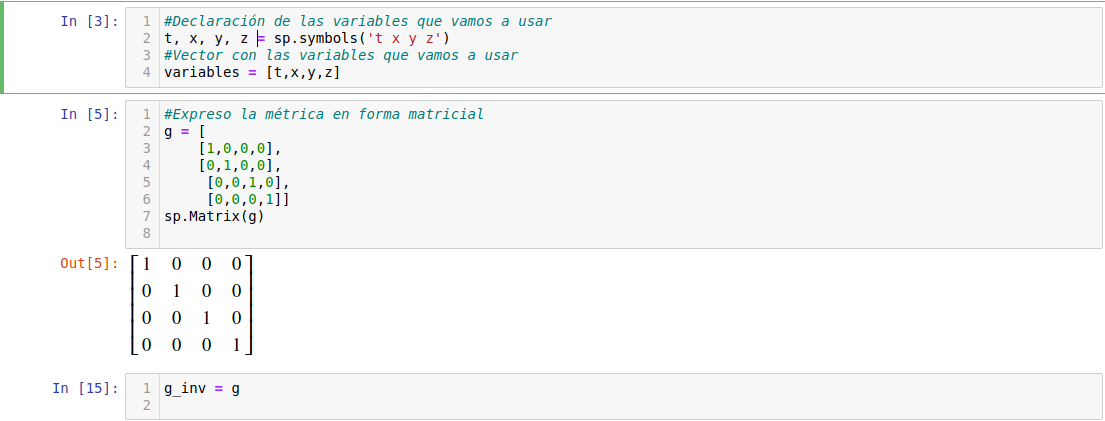
\includegraphics[scale = 0.33]{euclidea_declaracion.png}
    \caption{Declaración de las variables que se van a usar en la métrica euclidea }
    \label{fig:euclidea_declaracion}
\end{figure}
\newpage
Posteriormente, se calculan las derivadas covariantes de las componentes de la matriz y lo almacenamos en una matriz, como se ha explicado en la sección anterior y como se puede ver en la figura \ref{fig:euclidea_covariante}. Como era de esperar todos las derivadas covariantes son nulas y por lo tanto todos los símbolos de Christoffle son nulos también. 

\begin{figure}[!ht]
    \centering
    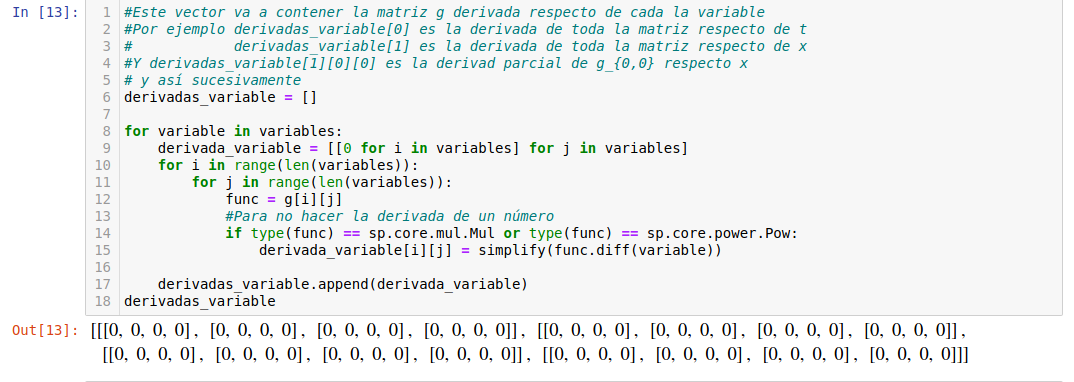
\includegraphics[scale=0.33]{euclidea_covariante.png}
    \caption{Calculo de las derivadas covariantes de la matríz de la métrica euclidea}
    \label{fig:euclidea_covariante}
\end{figure}

Y finalmente calculamos las geodésicas 

\newpage






\subsection{Métrica de Poincaré}
Como se mostró en la sección  la métrica de Poincaré es: 
\begin{equation}
    ds= \frac{dx \otimes dx + dy \otimes dy}{y^2}
\end{equation}



Y su expresión matricial es: 
\begin{equation}
    \left[\begin{matrix}\frac{1}{y^{2}} & 0\\0 & \frac{1}{y^{2}}\end{matrix}\right]
\end{equation}
Entonces con el programa que se ha mostrado antes obtenemos que que los símbolos de Christoffel son: 
\begin{equation}
    \Gamma^x_{x,x}= \Gamma^x_{y,y} = \Gamma^y_{x,y} = \Gamma^y_{y,x} = 0
\end{equation}
\begin{equation}
    \Gamma^x_{x,y} = \Gamma^x_{x,y}  = \Gamma^y_{y,y}=  \frac{-1}{y} 
\end{equation}

\begin{equation}
    \Gamma^y_{x,x} = \frac{1}{y}
\end{equation}
Introducción a la Información, Computación y Algorítmica Cuántica (105000346)
Y obtenemos que las geodésicas tienen la siguiente forma: 
\begin{equation}
\begin{array}{l}
\frac{d}{d \tau} d x(\tau)-\frac{2 \mathrm{dx}(\tau) \mathrm{dy}(\tau)}{y}=0 \\
\frac{d}{d \tau} \mathrm{dy}(\tau)+\frac{\mathrm{~d} \mathrm{x}^{2}(\tau)}{y}-\frac{ \mathrm{dy}^{2}(\tau)}{y}=0
\end{array}
\end{equation}



\subsection{Métrica de Schwarzschild}
La métrica de Schwarzschild es una creada por Karl Schwarzschild en 1916 como solución a las ecuaciones de Einstein. Esta solución presenta  un atractor en el centro del sistema de coordenadas. 
Esta métrica expresada en coordenadas esféricas es de la siguiente forma: 
\begin{equation}
    ds^2= -(1-2M/)
\end{equation}


En Schwarzschild el tiempo cuando un observador se acerca a $r_s$ se dilata tanto que parece que está parado \url{https://jila.colorado.edu/~ajsh/bh/schwp.html}




\chapter{Conclusiones}




% ------------------- Bibliografia ---------------------




\begin{thebibliography}{}
\bibliographystyle{plain}
\bibitem{nomograma} Dongsheng Yang. Build Prognostic Nomograms for Risk Assessment Using SAS.

\bibitem{boothby} W. M. Boothby An introduccion to differentiable manifolds and riemannian geometry 

\bibitem{DoCarmoRiemann} do Carmo, M.P. Riemannian Geometry 1992 Birkh{\"a}user.

\bibitem{gondinho} L. Gondinho y J. Natario An Introduction to Riemannian Geometry With Applications to Mechanics and Relativity

\bibitem{Fomenko} A. Mishchenko y A. Fomenko A course of Differential Geometry and Topology. 1988 Mir. 

\bibitem{algebralineal} Gabriela Jeronimo, Juan Sabia y Susana Tesauri Apuntes Álgebra Linea,2008 Universidad Buenos Aires.

\bibitem{chamizo} Fernando Chamizo, Apuntes del curso de Geometría y topología impartido durante el curso 2016/2017 en la Universidad Autónoma de Madrid. \url{https://github.com/apuntes-uam-infomat/apuntes/blob/master/Geometria%20y%20Topologia/GeoTopo17.pdf} 
\bibitem{WinterSchool}The WE-Heraeus International Winter School on Gravity and Light. (2015, February 10). Lecture 5: Tangent Spaces (International Winter School on Gravity and Light 2015) [Video]. YouTube. \url{https://www.youtube.com/watch?v=pepU_7NJSGM}


\end{thebibliography}
% ------------------- Anexos ---------------------

\appendix
\renewcommand\appendixname{Anexo}

% ---- Primer Anexo ----
\chapter{Código Nomograma}
\label{anexo:codigonomograma}
\begin{minted}
[
frame=lines,
framesep=5mm,
baselinestretch=1,
linenos
]{python}

import pandas as pd
import numpy as np

from IPython.display import HTML


import saspy as sp
import os
os.environ["PATH"] += ";C:\\Program Files\\SASHome\\SASFoundation\\9.4\\core\\sasext"

def sacar_tablas():


    es_correcto = False
    print("Los números se deben de introducir en formato americano (X.Y)")
    while not es_correcto:
        numero_variables = int(input("Introduce el número de Variables:\t"))
        es_correcto =  True if input("¿Los datos son correctos?(S/N) ").upper() == 'S'
 else False

    i = 0
    #Este diccionario en este paso va a almacenar la variable junto con
# si es categórica o no, y luego cada nivel, con
    # su valor del beta y el absolute beta value
    # se identificara con 0 una variable categórica
   #Se indentificara con 1 una variable contínua
    diccionario_variable = {}
    diccionario_max_min = {}

    variables =[]
    betas=[]
    v_var_global = []
    es_correcto = False
    while not es_correcto:
        intercept = float(input("Introduce el estimador intercept:\t"))
        es_correcto =  True if input("¿Los datos son correctos?(S/N) ").upper() == 'S' else False

    betas.append(intercept)
    while i < numero_variables:
        #Para no tener que meter todo otra vez
        correcto = False
        while not correcto:
            nombre_variable = input("Introduce el nombre la variable: \t")
            nombre_variable = nombre_variable.replace(" ", "_")
            es_categorica = -1
            while es_categorica not in [0,1]:
                try:
                    es_categorica = int(input("¿La variable es categórica?\n\t0 si es
 categórica \n\t1 si es contínua\n"))
                except:
                    print("El formato no es válido vuelva a introducirlo otra vez
(Debe ser un número en formato americano X.Y)")
                if es_categorica not in [0,1]:
                    print("Clase de la variable introducida no es correcto. 
Por favor vuelva  a introducirlo")

            vector_info_variable = [es_categorica]
            vector_beta_variable = []
            vector_variables_variable = []
            max_min_var = []



            #Si es categorica
            if es_categorica == 0:
                numero_niveles = int(input("Introduce el número de niveles:\t"))
                j  = 0
                while j < numero_niveles:
                    nombre_nivel = input("Introduce el nombre del nivel:\t")
                    try:
                        estimador_beta = float(input("Introduce el estimador para dicho parametro:\t"))
                    except:
                        print("El formato no es válido vuelva a introducirlo otra vez")
                        estimador_beta = float(input("Introduce el estimador para dicho parametro:\t"))

                    vector_variables_variable.append(nombre_nivel)
                    vector_beta_variable.append(estimador_beta)
                    vector_info_variable+= [nombre_nivel, estimador_beta, estimador_beta]

                    j+= 1
            #Si es contínua
            else:
                try:
                    estimador_beta = float(input("Introduce el estimador para dicho parametro:\t"))
                except:
                    print("El formato no es válido vuelva a introducirlo otra vez")
                    estimador_beta = float(input("Introduce el estimador para dicho parametro:\t"))
                try:
                    minimo =float(input("Introduce el minimo de dicha variable:\t"))
                except:
                    print("El formato no es válido vuelva a introducirlo otra vez")
                    minimo =float(input("Introduce el minimo de dicha variable:\t"))
                try:
                    maximo = float(input("Introduce el maximo de dicha variable:\t"))
                except:
                    print("El formato no es válido vuelva a introducirlo otra vez")
                    maximo = float(input("Introduce el maximo de dicha variable:\t"))

                max_min_var = [maximo, minimo]

                vector_info_variable += [ estimador_beta, estimador_beta*(maximo-minimo),
            sestimador_beta*(maximo-minimo)]
                #vector_info_variable += [ estimador_beta, estimador_beta*(maximo),estimador_beta*(maximo)]
                vector_beta_variable.append(estimador_beta)
                vector_variables_variable.append(nombre_variable)

            correcto =  True if input("¿Los datos son correctos?(S/N)").upper() == 'S' else False
            if correcto:
                break
            else:
                print("Introduce otra vez los datos")
        betas += vector_beta_variable
        variables += vector_variables_variable
        diccionario_variable[nombre_variable] = vector_info_variable
        v_var_global.append(nombre_variable)
        if es_categorica == 1:
            diccionario_max_min[nombre_variable]  = max_min_var
        i+=1
        print("")
    dict_variables_unidas = diccionario_variable

    #Si todos son negativos lo invertimos
    betas_todos_neg= [1 if i < 0 else 0 for i  in betas]

    todos_neg = False
    if 1 in betas_todos_neg[1:] and not 0 in betas_todos_neg[1:] and len(betas) > 2:
        todos_neg = True
        copia_betas = [i for i in betas]
        betas =[betas[0]] + [abs(betas[i]) for i in range(1, len(betas))]




    asociacion = [(variables[i],betas[i +1]) for i in range(len(variables))]

    #Diccionario_variables es un diccionario que
# emparaja cada variable de la regresión con su beta
    #Lo que hago con (len(betas)-len(variables) 
#es para la diferencia de quitar todos los intercept que aparecen. s
    diccionario_variables = {asociacion[i][0]:
[asociacion[i][1]] for i in range(0,len(asociacion))}


    #Ordeno las variables según su absolute beta value maximo
    v = []
    #Aquí hay que poner el abs() si no funciona

    for var in v_var_global:
        v.append((var,max([i for  i in dict_variables_unidas[var][3::3]])))

         #Prueba con el abv  que no sea absolute porque puede ocurrir que los betas sean negativos
    #Como dice el artículo:
    v_var_global.sort(key= lambda var: max( 
[i for i in dict_variables_unidas[var][3::3]]), reverse = True)
    #v_var_global.sort(key= lambda var: max(
 [i for i in dict_variables_unidas[var][3::3]]), reverse = True)


    #Seleccionamos la que mayor ABV tiene:
    max_var = v_var_global[0]
    tipo_max_var = dict_variables_unidas[max_var][0]

    #Saco los Maximos LP y los mínimos LP
    #Si es contínua
    if tipo_max_var == 1:
        #Saco el beta asociado a esa variable
        beta_continua =  dict_variables_unidas[max_var][1]


        #Calculo sus maximos predictores lineales
        max_LP = beta_continua*diccionario_max_min[max_var][0]
        min_LP = beta_continua*diccionario_max_min[max_var][1]

    #Si es categorica siempre va a estar como 0 o 1
    else:

        #Calculo los LP

        vector_beta = [v for v in dict_variables_unidas[max_var][2::3]]

        max_LP = max(vector_beta)* 1

        #Si es categórica siempre va a ser 0 porque es el mínimo
        min_LP = 0

    puntos_por_unidad_de_lp = 100/(max_LP-min_LP)

    print(max_LP, min_LP)

    suma_min_abs = abs(betas[0])
    suma_min =betas[0]
    for variable in v_var_global:
        #Si es continua
        print(variable,dict_variables_unidas[variable][0] )
        if dict_variables_unidas[variable][0] == 1:

            suma_min += dict_variables_unidas[variable][1]
*diccionario_max_min[variable][1]

            suma_min_abs += abs(dict_variables_unidas[variable][1])
*diccionario_max_min[variable][1]
        else:

            vector_beta = [v for v in dict_variables_unidas[variable][2::3]]
            #Si solo es de 0, 1
            if len(vector_beta) == 1:
                suma_min += 0
            else:
                suma_min += min(vector_beta)
                suma_min_abs += abs(min(vector_beta))

    suma_max =  betas[0]
    suma_max_abs= abs(betas[0])
    for variable in v_var_global:
        #Si es continua
        if dict_variables_unidas[variable][0] == 1:
            suma_max += dict_variables_unidas[variable][1]
*diccionario_max_min[variable][0]
            suma_max_abs +=abs(dict_variables_unidas[variable][1]
* diccionario_max_min[variable][0])
        #Si es categórica
        else:
            vector_beta = [v for v in dict_variables_unidas[variable][2::3]]
            suma_max += max(vector_beta)
            suma_max_abs += abs(max(vector_beta))

    escritor_salida = open("nomograma.txt","w")
    escritor_salida.write("y	y_label	x_label	x	low	
high	x_label2\n")

    #Saco los totalpoints
    #
    if tipo_max_var == 1 :
        min_total_points =  puntos_por_unidad_de_lp * (min_LP-min_LP)
        max_total_points =puntos_por_unidad_de_lp  *(max_LP-min_LP)
    else:
        min_total_points = (puntos_por_unidad_de_lp * 
(suma_min - (betas[0])))
        max_total_points =(puntos_por_unidad_de_lp  *
(suma_max -(betas[0])))#(puntos_por_unidad_de_lp  *
(suma_max_abs- abs(betas[0])))


    min_risk_of_y = np.e**(suma_min)/(1+np.e**(suma_min))
    max_risk_of_y = np.e**(suma_max)/(1+np.e**(suma_max))

    inicio_bucle = min_risk_of_y
    fin_bucle =max_risk_of_y


    #Primero escribo las tablas risk of even total points
    cadena_risk_of_event = ""
    #Para que comience en el siguiente
    partes = 7
    pos = 1

    if not todos_neg:
        i = ( inicio_bucle+betas[0])/puntos_por_unidad_de_lp
        cadena_risk_of_event = "{}\t {}\t {:2.2f}\t {:2.2f}\t
 {}\t {}\t {}\n".format(1,"Risk of Event",
 min_risk_of_y,0, 0.9,1, "")

        cadena_total_points = "{}\t {}\t {:2.2f}\t {:2.2f}\t
 {}\t {}\t {}\n".format(2,"Total Points", 
round(min_total_points),0, 1.9,2, "")

        partes = 7
        pos = 1

        lp= min_total_points + (max_total_points -
 min_total_points)/partes 

        while  lp < abs(max_total_points):
            puntos = (lp)/puntos_por_unidad_de_lp+betas[0]
+len(v_var_global)*min_LP#len(diccionario_max_min.keys())*min_LP
            risk_of_y = np.e**puntos/(1+np.e**puntos)
            total_point =  lp
            x_label2 = ""
            #       y y_label x_label x low 
high x_label
            cadena_risk_of_event += "{}\t {}\t {:2.2f}\t {:2.2f}\t {}\t {}\t {}\n".format(1,
"Risk of Event", round(risk_of_y,2),pos/(partes+1)*100, 0.9,1, x_label2)

            cadena_total_points += "{}\t {}\t {:2.2f}\t {:2.2f}\t {}\t {}\t {}\n".format(2,
"Total Points", round(total_point),pos/(partes+1)*100, 1.9,2, "")

            lp += (max_total_points - min_total_points)/(partes+1)#(abs(max_total_points) - 
abs(min_total_points)).7
            pos += 1

        puntos = (lp)/puntos_por_unidad_de_lp+betas[0]
        risk_of_y = np.e**puntos/(1+np.e**puntos)

        cadena_risk_of_event  += "{}\t {}\t {:2.2f}\t {:2.2f}\t {}\t {}\t {}\n".format(1
"Risk of Event", max_risk_of_y,100, 0.9,1, "")

        cadena_total_points+= "{}\t {}\t {:2.2f}\t {:2.2f}\t {}\t {}\t {}\n".format(2,
"Total Points",round(max_total_points) ,100, 1.9,2, "")

    #Si todos los betas son negativos le damos la vuelta a la cadena de risk of  event
    else:
        i = ( inicio_bucle+betas[0])/puntos_por_unidad_de_lp
        cadena_risk_of_event = "{}\t {}\t {:2.2f}\t {:2.2f}\t {}\t {}\t {}\n".format(1,
"Risk of Event",max_risk_of_y,0, 0.9,1, "")

        cadena_total_points = "{}\t {}\t {:2.2f}\t {:2.2f}\t {}\t {}\t {}\n".format(2,
"Total Points", round(min_total_points),0, 1.9,2, "")
        partes = 7
        pos = 1
        #bulce para total points
        incremento = (max_total_points - min_total_points)/partes
        lp = min_total_points + incremento
        while lp < max_total_points:
            total_point = lp
            x_label2 = ""
            cadena_total_points += "{}\t {}\t {:2.2f}\t {:2.2f}\t {}\t {}\t {}\n".format(2,
"Total Points",  round(total_point),pos/(partes+1)*100, 1.9,2, "")

            pos += 1

            lp += incremento


        #bucle del risk of y
        pos = 1
        incremento = (max_risk_of_y - min_risk_of_y)/partes
        riesgo = max_risk_of_y - incremento

        while riesgo > (min_risk_of_y+incremento):
            x_label2 = ""
            cadena_risk_of_event += "{}\t {}\t {:2.2f}\t {:2.2f}\t {}\t {}\t {}\n".format(1,
"Risk of Event", 
round(riesgo,2),pos/(partes+1)*100, 0.9,1, x_label2)
            riesgo -= incremento
            pos += 1

        cadena_risk_of_event += "{}\t {}\t {:2.2f}\t {:2.2f}\t {}\t {}\t {}\n".format(1
,"Risk of Event", 
round(min_risk_of_y,2),pos/(partes+1)*100, 0.9,1, x_label2)

        cadena_total_points += "{}\t {}\t {:2.2f}\t {:2.2f}\t {}\t {}\t {}\n".format(2,
"Total Points",  round(max_total_points),pos/(partes+1)*100, 1.9,2, "")

    escritor_salida.write(cadena_risk_of_event)
    escritor_salida.write(cadena_total_points)


    y = 3
    for variable in v_var_global:

        datos_var = dict_variables_unidas[variable]

        tipo = datos_var[0]


        #Si la variable es numerica
        if tipo == 1:
            beta = datos_var[1]
            print(beta)
            maxi =diccionario_max_min[variable][0]
            mini =diccionario_max_min[variable][1]

            variable_contenido = mini
            incremento = (maxi-mini)/10

            for  n in range(0, 11):
                n= (n+1)*10

                lp = variable_contenido*beta

                x = round(100*(lp-min_LP)/(max_LP-min_LP))
                y_label = variable
                x_label = variable_contenido
                low = y -0.1
                high = y
                x_label2 = ""
                if n == 100 and beta < 0 and diccionario_max_min[variable][0]>0 and 
diccionario_max_min[variable][1]>0:
                    x_label2 = "Substract"
                variable_contenido += incremento
                #       y y_label x_label x low high x_label

                cadena = "{}\t {}\t {:2.2f}\t {:2.2f}\t {}\t {}\t {}\n".format(y, y_label,
 x_label, abs(x), low, high, x_label2)
                escritor_salida.write(cadena)
        # Si es categorica
        if tipo == 0:
            vector_info = datos_var[1:]
            nombres_categorias = vector_info[0::3]
            betas = vector_info[1::3]
            categoria = 0
            #Si solo tiene dos niveles
            if len(nombres_categorias) == 2:
                beta = betas[0]
                low = y -0.1
                high = y
                y_label = variable
                nombre_etiqueta = dict_variables_unidas[variable][1::3]
                #Con la puntuación 0
                x =  round(100*(beta-min_LP)/(max_LP-min_LP))
                x_label2 =nombre_etiqueta[0]
                x_label = ""
                cadena = "{}\t {}\t {}\t {:2.2f}\t {}\t {}\t {}\n".format(y, y_label,
 x_label.replace(" ", ""),abs(x), low, high, x_label2.replace(" ", ""))
                escritor_salida.write(cadena)

                #Con la puntuacion 1
                beta =betas[1]
                x =   round(100*(beta-min_LP)/(max_LP-min_LP))
                if beta < 0:
                    x_label2 = "Substract"
                else:
                    x_label2 = "Add"

                x_label = nombre_etiqueta[1]
                cadena = "{}\t {}\t {}\t {:2.2f}\t {}\t {}\t {}\n".format(y, y_label, 
x_label.replace(" ", ""),abs(x), low, high, x_label2.replace(" ", ""))
                escritor_salida.write(cadena)

            else: #Si tiene mas de dos niveles
                nombre_etiqueta = dict_variables_unidas[variable][1::3]
                nombre = nombre_etiqueta[0]
                #Para la variable de referencia
                escritor_salida.write("{}\t {}\t {}\t {:2.2f}\t {}\t {}\t {}\n".format
(y,variable,  nombre.replace(" ", ""),0, y-0.1, y, ""))
                while (categoria) < (len(vector_info)//3):
                    #Nombre de la categoria
                    cat  =nombre_etiqueta[categoria]
                    beta = betas[categoria]

                    x =round(100*(beta-min_LP)/(max_LP-min_LP))

                    x_label = cat
                    low = y -0.1
                    high = y
                    y_label = variable
                    x_label2 = ""
                    x_label = cat
                    if beta < 0 :
                        x_label2 = "Substract"
                    else:
                        x_label2 = "Add"

                    if x == 0:
                        x_label2 =cat
                        x_label = ""
                        if beta < 0:
                            x_label = "Substract"
                        else:
                            x_label = "Add"
                    cadena = "{}\t {}\t {}\t {:2.2f}\t {}\t {}\t {}\n".format(y, y_label, 
x_label.replace(" ", ""),abs(x), low, high, x_label2.replace(" ", ""))
                    escritor_salida.write(cadena)
                    categoria += 1
        y+= 1
    #Ahora rellenamos la variable de control

    categoria = "Points"
    for n in range(0, 11):
        n = 10*n
        y_label = categoria
        x_label = n
        x= n
        low = y-0.1
        high = y
        x_label2 = ""
        cadena = "{}\t {}\t {}\t {}\t {}\t {}\t {}\n".format(y, y_label, x_label, x, low, 
high, x_label2)
        escritor_salida.write(cadena)
    escritor_salida.close()
    return v_var_global


def leer_datos_completos(nombre_fichero="datos.txt"):
    try:
        fichero = open(nombre_fichero, "r")
    except:
        print("No existe el fichero", nombre_fichero)
        fichero = input("Por favor introduzca el nombre del fichero que contiene los datos: ")
    #Leemos la cabezera
    cabezera = fichero.readline()
    cabezera = cabezera[:-1]
    cabezera.replace(" 	", "	")
    fichero.close()

    data = pd.read_csv(nombre_fichero, sep="	")
    data.columns= [uwu.upper() for uwu in cabezera.split("	")]


    return data

def crear_nomograma(variables_orden, dir):
    nomograma = leer_datos_completos("nomograma.txt")

    proc_format = "proc format; \n value yfmt \n"
    fin = "2 = 'TOTAL POINTS' \n 1 = 'RISK' \n 0 = ' ';"
    for i in range(len(variables_orden), -1, -1):
        if i == len(variables_orden):
            proc_format += "{} = '{}'\n".format(i+3, "POINTS" )
        else:
            proc_format += "{} = '{}'\n".format(i+3, variables_orden[i] )
    proc_format += fin


    leer = """ data WORK.kkk    ;
    %let _EFIERR_ = 0; /* set the ERROR detection macro variable */
    infile 'nomograma.txt' delimiter='09'x MISSOVER DSD lrecl=32767 firstobs=2 ;
       informat y best32. ;
       informat y_label $15. ;
       informat x_label $10. ;
       informat x best32. ;
       informat low best32. ;
       informat high best32. ;
       informat x_label2 $10. ;
       format y best12. ;
       format y_label $15. ;
       format x_label $10. ;
       format x best12. ;
       format low best12. ;
       format high best12. ;
       format x_label2 $10. ;
    input
                y
                y_label $
                x_label $
                x
                low
                high
                x_label2 $
    ;
    if _ERROR_ then call symputx('_EFIERR_',1);  /* set ERROR detection macro variable */
    run;\n
 """
    proc_sgplot = r"ods graphics on/ imagefmt=svg imagename='SVG';" +"\n" + r" ODS LISTING GPATH = 
'C:\Users\fgonzalez\Desktop\mis_proyectos\nomograma\UntitledFolder\libreria_python' ;"+ "\n"
+ " proc sgplot data 
= kkk noautolegend ;"+ "\n" +"  series x = x y = y/group = y_label  lineattrs = (pattern = 
1 thickness = 2);"+ "\n"+ " 
 highlow x=x high = high low=low / lowlabel=x_label  highlabel=x_label2;  yaxis display= 
( nolabel noline noticks )
 tickvalueformat =yfmt. VALUES=(0 TO {} BY 1);".format(len(variables_orden)+3)+"\n"+ " 
 xaxis display= none ; run;"
    subir = leer + proc_format + proc_sgplot


    escritor_fichero_sas = open(r"{}\Nomograma.sas".format(dir), "w")
    escritor_fichero_sas.write(subir)
    escritor_fichero_sas.close()
    try:
        sas =sp.SASsession(cfgname='winlocal', results='Pandas', encoding='utf-8')
        codigo_sas = open(r"{}\Nomograma.sas".format(dir), "r")
        codigo = codigo_sas.read()

        return_sas = sas.submit(codigo)
        codigo_sas.close()
    except:
        print("Debes de instalar la librería SASPy, pero se ha creado un archivo .sas que
 contiene el código para ejecutarlo.")
        return False

    return True


variables_orden= sacar_tablas()

dir = os.getcwd()
v = crear_nomograma(variables_orden, dir)
print(v)

\end{minted}

\chapter{Estructuras maximales}\label{apend.B}
En este apéndice se demostrará que toda estructura diferenciable que no sea maximal existe una estructura diferenciable maximal a la que pertenece.


\begin{propo} Sea \M un espacio Hausdorff y 2AN. Sea $\mathscr{V}$ = \{($V_\beta, \phi_\beta $)\}$_{\beta \in I}$ un recubirmiento de \M y un entorno coordenado \Cinf -compatibles. Entonces existe una única estructura de clase \Cinf diferenciable en \M que contiene a este entorno coordenado.
\end{propo}

\begin{proof}

Para probar que existe una variedad que contiene a $\mathscr{V}$ se va a construir una estructura diferenciable compatible con \M. $\mathscr{U}=\{(U_i, \psi_i)\}_{i \in I'}$ de modo que son una familia de todos los entornos coordenados de \M  de \Cinf-compatibles con cada uno de los $(V_\beta, \psi_\beta)$ .

Una vez definido $\mathscr{U}$ se va a demostrar, siguiendo la definición \ref{def:variedad_dif}, que es una estructura diferenciable de \M. 
\begin{enumerate}
\item $\bigcup_{i \in I}U_i=$\M debido a que $\mathscr{U}$ contiene a  $\mathscr{V}$ y este recubría a \M.
\item Ahora vamos a ver que cumple la segunda propiedad. Para ello vamos a tomar dos entornos coordenados $(U_i, \psi_i)$ y $(U_i', \psi_i') $ que pertence a $\mathscr{U}$ y $U' \cap U \neq \emptyset$, entonces tenemos que ver que $\forall \alpha, \beta \in I'$: 
	\begin{itemize}
		\item $ \psi_i(U_i) \bigcap \ \psi_i'(U_i') = W \neq \emptyset$ Tal y como hemos definido nuestra familia de entornos coordenados tenemos que son cambios de coordenadas y homeomorfismos bien definidos de abiertos de \R$^n$
		\item Como hemos dicho en el punto anterior tenemos que son cambios de coordenadas y por lo tanto $\psi_i^{-1}(U_i)$ y $\psi_i'^{-1}(U'_i)$ son abiertos de \R$^n$
		
		\item Ahora nos falta demostrar que $\psi_i \circ \psi_i' $ es diferenciable. Sea x = $\psi(x)\in \psi(U \bigcap U')$ entonces tenemos que $p\in V_\beta$ para uno de los entornos coordenados de $\mathscr{V}$. Por lo tanto hay un abierto W tal que $p \in W =V_\beta \bigcap U \bigcap U'$ y $x \in \psi(W)$, que también es abierto. Entonces tenemos que $\psi_i \circ \psi_i'= \psi_i \circ \phi^{-1}_\beta \circ \phi_\beta \circ \psi_i'  $ en $\psi(W)$ pero como $(U_i, \psi_i)$ y $(U_i', \psi_i') $ con \Cinf -compatibles con ($V_\beta, \phi_\beta $) entonces $ \psi_i \circ \phi^{-1}_\beta$ y $ \phi_\beta \circ \psi_i'$ son diferenciables  y por ende $\psi_i \circ \psi_i'$ también lo es en $\psi(W)$. Y en consecuencia se obtiene que es diferenciable en todo entorno coordenado de su dominio. 
	\end{itemize}
	
	
\item Esta propiedad es directa debido a que para cualquier (U, $\psi$) que sea compatible con todos los entornos coordenados de la familia que hemos construido; en concreto lo es respecto la familia inicial $\mathscr{V}$.
\end{enumerate}
Y por lo tanto $\mathscr{U}=\{(U_i, \psi_i)\}_{i \in I'}$ es una estructura diferenciable maximal.
\cite{boothby}
\end{proof}

\chapter{Runge Kutta Orden 4}\label{Apend.C}
\begin{minted}[
frame=lines,
framesep=5mm,
baselinestretch=1,
linenos
]{python}


# metodo de Runge-Kutta de orden 4 para un sistema de N eqs


import os


#La función como tal
def f(j, x):
    #j nos indica si queremso el 0 o el 1
    #x[0]=x y x[1]=y
    resultado = 0


    #En el caso de que haya mas de 2 dimensiones añadir un elif
    if j == 0:
        try:

            resultado +=  x[2]
        except:
            print("Overflow error")
            return
    elif j == 1:
        try:

            resultado += x[3]
        except:
            print("Overflow error")
            return
    elif j == 2:
        try:
            resultado = 2*(x[2]*x[3])/x[1]
        except:
            print("Overflow error")
            return
    else:
        try:

            resultado = (-x[2]**2+x[3]**2)/x[1]
        except:
            print("Overflow error")
            return
    return resultado


def F(i, j , x, w, dim, h):
    #dim es la dimensión
    # h es el paso
    r = [0 for a in range(dim)]
    v = 0

    if i == 0:
        for a in range(0, dim):
            r[a] = x[a]

    elif i == 1 or i == 2:
        for a in range(dim):
            r[a] = x[a]+ (h/2)* w[i-1][a]
    else: #si es 3
        for a in range(dim):
            r[a] = x[a] + h*w[i-1][a]

    v = f(j, r)
    return v



def main():

    N = 4 # el tamaño del espacio de estados

    y= [0 for i in range(N)]

    w = [[0 for j in range(N)] for i in range(0,4)]

    k = 0

    print("Introducir tiempo máximo:")
    t= 0
    #tmax = int(input())
    tmax=100

    #Leo los datos iniciales
    for j in range(0, N):
        print("Introduce x[{}]:\t".format(j))
        y[j] = float(input())

    #Introducir el paso temporal un buen h = 0.001
    print("Introduce el paso temporal: \t")
    h = float(input()) #Puede ser positivo o negativo
    #h= 0.001
    #creo y abro el fichero de salida
    nombre_fichero = "datospython{}-{}.dat".format(y[0], y[1])
    fichero_salida = open(nombre_fichero, 'w')
    fichero_salida.write("# metodo de R-K segun rk.c \n")

    #Escribo el punto inical
    esc = "{:20.20f}".format(t)
    fichero_salida.write(str(esc))

    for d in y:
        fichero_salida.write("\t {:20.20f}".format(d))
    fichero_salida.write("\n")
    #Iteraciones de Runge-Kutta
    while abs(t) < tmax:

        k += 1
        #Aumento el tiempo
        t += h


        #coeficientes del método RK
        for i in range(0, 4):
            for j in range(0, N):
                w[i][j] = F(i, j, y, w, N, h)
                if w[i][j] is None:
                    fichero_salida.close()
                    return

        #escribo el tiempo
        esc = "{:20.20f}".format(t)
        fichero_salida.write(str(esc))

        #Solucion numerica
        for j in range(0, N):
            y[j] += (w[0][j] + 2*(w[1][j] + w[2][j]) + w[3][j]) * h/6
            res_aux = "\t {:20.20f}".format(y[j])
            fichero_salida.write(res_aux)
        fichero_salida.write("\n")
        if y[1]<10**-5:
            break
    #Cierro el fichero
    fichero_salida.close()

    return


if __name__ == "__main__":
    main()
\end{minted}

\end{document}

